\documentclass[10pt,a4paper]{article}
\usepackage{mystyle}

\begin{document}

\maketitle
\vfill
% Abstract
\section*{Abstract}

I \textit{Monads} sono un'importante strumento per i linguaggi funzionali.
Differenti \textit{Monads} possono essere utilizzati per modellare
un ampio gruppo di features di programmazione.
Vedremo come questi meccanismi portino benefici in un semplice esempio.
Molto spesso progetti di qualsiasi entità richiedono combinazioni di queste
feature, è quindi importante avere tecniche per poter combinare varie
\textit{Monads} in un singolo \textit{Monad}.
In pratica questa non è un'operazione difficile, infatti è
possibile combinare qualche feature specifica per costruire nuovi
\textit{Monads} con facilità.
Le tecniche solitamente utilizzate però sono generalmente ad-hoc e sembra molto
più difficile il problema di trovare una caratterizzazione generale per
combinare \textit{Monads} in maniera arbitraria.
Vedremo poi tre costrutti generali per comporre \textit{Monads}, ognuno di esso
collegato alle proprie condizioni e funzioni ausiliarie.
Concludendo con un esempio pratico.
\clearpage
\tableofcontents
\clearpage


%-------------------------------------------------------------------------------

% \begin{center}

%   \footnotesize
%   \begin{tabular}{>{\itshape}l>{\itshape}l}
%     \multicolumn{2}{l}{-- Using a generator function}\\
%     fib n & fibs (0,1) !! n \\
%           \begin{align}
%           where & fibs (a,b) = a : fibs (b,a+b)\\
%             &  a = 0\\
%           \end{align}
%     \end{tabular}
%   \end{center}
% \begin{center}
% \begin{blstlisting}
%   JoinP  $=$  s
%   JoinP  ::s
% \end{blstlisting}
% \end{center}

% \begin{align*}
% joinP &{}={} PComposable ...\\
% joinP &{}:: join ... &{}= another \\
% \end{align*}

%-------------------------------------------------------------------------------

% Introduction
\section{Introduction}

Recentemente, il concetto di Monade è diventato un importante e pratico
strumento per i linguaggi funzionali.
La ragionde di questo dipende dal fatto che i \textit{Monads} propongono un
framework uniforme per descrivere una enorme set di caratteristiche tipicamente
imperative all'interno di un sistema puro.\\
Nella sezione \ref{a_simple_evaluator} vedremo una possibile implementazione per
una funzione di valutazione di una semplice grammatica, esplicitando tutta la
computazione necessaria.\\
L'introduzione ai \textit{Monads} è definita nel capitolo \ref{monads}, dove
definisco la struttura di un Monade e ne descrivo le proprietà.\\
Successivamente, la sezione \ref{monadic_evaluator}, descrive lo stesso
interprete in chiave monadica, esponendo i vantaggi dell'applicazione delle
\textit{Monads} su questo semplice esempio.\\
La sezione \ref{composing_monads} pone le basi e descrive la caratterizzazione
generale del concetto di \textit{Composing Monads}, questa sezione non entra nel
dettaglio dell'algebra astratta ad alto livello, ma ragione su una astrazione
di un linguaggio funzionale puro. Questa è la sezione principale di questo
report, definendo formalmente le tre classi di possibili tecniche per combinare
\textit{Monads} in maniera arbitraria.\\
Passiamo poi a definire nella sezione \ref{general_framework_for_composition}
un sistema per generalizzare la composizione dei monadi.\\
L'ultima sezione (capitolo \ref{composed_monad_interpreter}) infine implementa
i meccanismi definiti nella sezione \ref{composing_monads} nello stesso esempio
visto nei primi due capitoli.\newline

Per questo report non assumo nessun linguaggio di programmazione, gli esempi e
la sintassi utilizzata fanno riferimento a \textit{Gofer}
\footnote{\textit{Gofer}, un piccolo, sperimentale e semplice linguaggio
puramente funzionale}, simile ad \textit{Haskell}.
In appendice \ref{scala_code} troviamo anche un pratico esempio in \textit{Scala} per la composizione
generalizzata.\newline

In appendice \ref{proofs} definisco le dimostrazioni che ritengo più importanti
e istruttive. Alcune dimostrazioni semplici e/o limitate sono definite tra le
righe, solitamente delimitate da un semplice box.
Mentre in appendice \ref{state_transformer} mostro un esempio di come un
\textit{composed monad} non riesce ad esprimere il concetto di
\textit{State Transitions}, per questo esempio noteremo come un'implementazione
ad-hoc sia diversa dall'equivalente rappresentazione mediante composizione.


\newpage

% Simple Evaluator
\section{A Simple Evaluator}
\label{a_simple_evaluator}

\subsection{Abstract Syntax} %--------------------------------------------------
\label{abstract_syntax}

La funzione di valutazione riceverà in input espressioni generate dalla seguente
grammatica:

\begin{figure}[h]
  \centering
  \footnotesize % adapt to your page size
  \begin{haskellsyntax}
  \mv{Expr} \STO \mv{Const} \ \mv{Value}
                  \REM{Valore costante}
            \SOR \mv{Var} \ \mv{Name}
                  \REM{Variabile in memoria}
            \SOR \mv{Expr} + \mv{Expr}
                  \REM{Addizione tra espressioni}
            \SOR \mv{Trace} \ \mv{String} \ \mv{Expr}
                  \REM{Struttura di log}
  \\
  \mv{Env} \STO [(\mv{Name}, \mv{Value})]
                \REM{Ambiente di mapping delle variabili}
  \\
  \mv{Name} \STO \mv{String}
  \\
  \mv{Value} \STO \mv{Int}
  \end{haskellsyntax}%

\end{figure}

Per mantere l'esempio semplice ho ridotto al minimo le espressioni generabili
nel linguaggio, permettendo solamente costanti, variabili, addizioni ed un
semplice meccanismo di log.\newline

Si noti come questa grammatica permetta comunque l'implementazione di alcune
caratteristiche basilari come: la gestione degli errori per variabili
sconosciute, un sistema di output e la gestione dell'accesso delle variabili nel
sistema.

\subsection{Implementation} %---------------------------------------------------
\label{implementation}

Per la prima implementazione della funzione di valutazione utilizzo i seguenti
tipi astratti:

\begin{figure}[h]
  \centering
  \footnotesize % adapt to your page size
  \begin{haskellsyntax}
  \textbf{data} \ Error \ a &= Error \ String \sor Ok \ a
  \\
  \textbf{data} \ Writer \ s \ a &= (s, a)
    \REM{con s $::$ \textit{Monoid}, vedi \ref{monoid}}

  \end{haskellsyntax}%

\end{figure}

Con questi due tipi riusciamo a codificare la gestione degli errori e la
gestione del log, per la codifica dell'\textit{Enviroments} definiamo
semplicemente la funzione di valutazione, che riceverà in input lo stato
iniziale e ritornerà un valore (se nessun errore è occorso) e un output,
possibilmente vuoto.

\begin{align*}
  eval :: Expr \to Env \to Writer \ [String] \ (Error \ Value)
\end{align*}

Già dal tipo della funzione \textit{eval} si può notare come sia poco pulito,
difatti il tipo di ritorno è molto complesso dato che deve gestire ben due
caratteristiche non banali, la gestione dell'output e degli errori.
Ora passiamo all'implementazione dell'interprete.

\begin{figure}[H]
  \centering
  \footnotesize % adapt to your page size
  \begin{haskellsyntax}
  eval \ (Const \ v) \ env &= ([\ ], \ Ok \ a)\\
  eval \ (Var \ x) \ env   &= ([\ ], \ lookup \ env \ x)\\
  eval \ (e_0 + e_1) \ env  &= \textbf{case} \ eval \ e_0 \ env \ \textbf{of}\\
                            {}& \qquad (out_0, \ Error \ s) \to ([\ ], \ Error \ s)\\
                            {}& \qquad (out_0, \ Ok \ v_0) \quad \to \textbf{case} \ eval \ e_1 \ env \ \textbf{of}\\
                            {}& \qquad \qquad (out_1, \ Error \ s) \to ([\ ], \ Error \ s)\\
                            {}& \qquad \qquad (out_1, \ Ok \ v_1) \quad \to (out_0 \doubleplus out_1, v_0 \textbf{+} v_1)\\
  eval \ (Trace \ s \ e) \ env  &= ([s], \ eval \ e \ env)
  \end{haskellsyntax}%
\end{figure}

Prima di procedere notiamo l'utilizzo della funzione \textit{lookup} definita come segue.

\begin{figure}[H]
  \centering
  \footnotesize % adapt to your page size
  \begin{haskellsyntax}
  lookup &:: Env \to Name \to Error\ Value \\
  lookup \ [\ ] \ x &= Error \ "Value \ unbounded"\\
  lookup \ [(name, \ value):xs] \ x &= \textbf{if} \ name = x \
                                          \textbf{then} \ Ok \ value \
                                          \textbf{else} \ lookup \ xs \ x
  \end{haskellsyntax}%
\end{figure}

Come possiamo notare questo interprete è complicato e necessita di esplicitare
tutti i passi computazionali esponendolo ad errori.
Il codice risulta meno mantenibile e ancora meno estensibile, un qualsiasi
cambiamento, o richiesta di nuova \textit{feature}, richiederebbe la modifica
di quasi la totalità delle righe di codice.
In un linguaggio imperativo banale l'implementazione di queste caratteristiche
è un task molto semplice e non richiede particolari competenze, i
\textit{Monads} serviranno proprio per portare questa facilità d'esecuzione
dentro ad un linguaggio funzionale puro.


\newpage


% Monads
\section{Monads}
\label{monads}

Walder\cite{walder0} definisce un \textit{Monad} come un tipo costrutture unario
\textit{M}, con un unico parametro, insieme alle tre funzioni \textit{map},
\textit{unit} e \textit{join} definite dal tipo

\begin{align*}
  map  &:: (a \to b) \to (M \ a \to M \ b) \\
  unit &:: a \to M \ a\\
  join &:: M\ (M \ a) \to M \ a
\end{align*}

Altre caratterizzazioni (equivalenti) possono essere definite per il concetto
dei \textit{Monads}, per esempio come definito in Walder\cite{walder1}

\begin{align*}
  bind :: M \ a \to (a \to M \ b) \to M \ b
\end{align*}

Ragionando su questa forma è semplice notare come sia del tutto equivalente alle
precedenti mediante le relazioni
\begin{align*}
  bind \ x \ f &= join \ (map \ f \ x)\\
  join\ x &= bind\ x\ id
\end{align*}

In ogni caso, per questo report, ho scelto di lavorare con \textit{map},
\textit{unit} e \textit{join} perchè rendono più marcata la differenza tra
\textit{Monads} e \textit{Premonads} e inoltre rendono più
semplice lo svolgimento delle dimostrazioni in questo framework.\newline

In aggiunta a queste funzioni si richiede di soddisfare una collezione di
proprietà algebriche

\begin{align*}
    map \ id &= id \law{M1} \\
    map \ f \ .\ map \ g &= map\ (f\ .\ g) \law{M2}\\
    unit\ .\ f &= map\ f\ .\ unit \law{M3}\\
    join\ .\ map\ (map\ f) &= map\ f\ .\ join \law{M4}\\
    join\ .\ unit &= id \law{M5}\\
    join\ .\ map\ unit &= id \law{M6}\\
    join\ .\ map\ join &= join\ .\ join \law{M7}
\end{align*}

Per lo scopo del report è conveniente definire per parti un \textit{Monad};
se \textit{M} è un tipo costruttore unario diremo che
\begin{enumerate}
  \item \textit{M} è un \textit{Functor} se c'è una funzione
    $map  :: (a \to b) \to (M \ a \to M \ b) $ che soddisfa le leggi
    \textit{(M1)} e \textit{(M2)}.
  \item \textit{M} è un \textit{Premonad} se c'è una funzione
    $unit :: a \to M\ a$ che soddisfa la legge \textit{(M3)}.
  \item \textit{M} è un \textit{Monad} se c'è una funzione
    $join :: M (M\ a) \to M\ a$ che soddisfa le leggi \textit{(M4)},
    \textit{(M5)}, \textit{(M6)} e \textit{(M7)}.

\end{enumerate}

% Monadic Evaluator
\section{Monadic Evaluator}
\label{monadic_evaluator}

Ora che sappiamo cosa siano i \textit{Monads} possiamo applicari al primo
esempio nella sezione \ref{a_simple_evaluator}, in questa sezione costruiremo un
valutatore monadico per rappresentare le caratteristiche volute.
Senza entrare troppo nel dettaglio divido l'esempio in due parti per semplicità,
nelle prossime sezione vedremo come combinare il tutto in maniera semplice ed
elegante con un sistema generalizzabile.

\subsection{Exceptions}
\label{exceptions}
Per rappresentare la gestione delle eccezioni definisco il \textit{Monad}

\begin{figure}[H]
  \centering
  \footnotesize % adapt to your page size
  \begin{haskellsyntax}
  \textbf{data}\ Exception\ a &= Raise\ String\ |\ Return\ a \\\\

  map &:: (a \to b) \to Exception\ a \to Exception\ b\\
  map\ f\ (Raise\ s) &= Raise\ s\\
  map\ f\ (Return\ x) &= Return\ (f\ x)\\\\

  unit &:: a \to Exception\ a\\
  unit &= Return\\\\

  join &:: Exception\ (Exception\ a) \to Exception\ a\\
  join\ (Raise\ s) &= Raise\ s\\
  join\ (Return\ x) &= x
  \end{haskellsyntax}%
\end{figure}
La dimostrazione la si può trovare in appendice \ref{exception_is_a_monad}.
Definiamo quindi il corrispondente interprete per la grammatica
\ref{abstract_syntax}
\begin{figure}[H]
  \centering
  \footnotesize % adapt to your page size
  \begin{haskellsyntax}
  eval &:: Expr \to Env \to Exception\ Value\\
  eval \ (Const \ v) \ env &= unit\ v\\
  eval \ (Var \ x) \ env   &= lookup \ env \ x\\
  eval \ (e_0 + e_1) \ env &= bind\ (eval\ e_0\ env)\\
                           & \qquad \lambda\ v_0 \to bind\ (eval\ e_1\ env)\\
                           & \qquad \qquad \lambda\ v_1 \to unit (v_0 + v_1)
  \end{haskellsyntax}%
\end{figure}
Nota se \textit{Exception }è \textit{Monad} posso usare sia join che bind,
per questo esempio è comodo utilizzare il bind operator.
Ora passiamo ad osservare i pregi di questo esempio, notiamo subito come il
codice sia più coinciso e descriva meglio l'intenzione piuttosto che la
computazione.
L'utilizzo di \textit{unit} e \textit{bind} semplifica sia l'implementazione che
il ragionamento sull'interprete rendendolo più resistente a possibili errori di
programmazione.

\subsection{Output}
\label{output}

Per l'output definiamo il tipo astratto \textit{Writer} che definisce un
meccanismo per tenere la traccia del log prodotto (se prodotto), richiedo
inoltre che il tipo di

\begin{figure}[H]
  \centering
  \footnotesize % adapt to your page size
  \begin{haskellsyntax}
    \textbf{data}\ Writer\ s\ a &= (s,\ a) \\\\

      map &:: Monoid\ s \Rightarrow (a \to b) \to Writer\ s\ a \to Writer\ s\ b\\
      map\ f\ (s,\ a) &= (s,\ f\ a)\\\\

      unit &:: Monoid\ s \Rightarrow a \to Writer\ s\ a\\
      unit\ x&= (zero,\ x)\\\\

      join &:: Monoid\ s \Rightarrow Writer\ s\ (Writer\ s\ a) \to Writer\ s\ a\\
      join\ (s',\ (s'',\ a)) &= (s' \doubleplus s'',\ a)
  \end{haskellsyntax}%
\end{figure}

Definiamo, come per le eccezioni, la funzione per la grammatica
\ref{abstract_syntax}

\begin{figure}[H]
  \centering
  \footnotesize % adapt to your page size
  \begin{haskellsyntax}
  eval &:: Expr \to Env \to Writer\ [String]\ Value\\
  eval \ (Const \ v) \ env &= unit\ v\\
  eval \ (Var \ x) \ env   &= \textbf{case}\ lookup \ env \ x\ \textbf{of}\\
                           & \qquad Raise\ s \to unit\ defaultValue\\
                           & \qquad Ok\ x \to unit\ x\\
  eval \ (e_0 + e_1) \ env &= bind\ (eval\ e_0\ env)\\
                           & \qquad \lambda\ v_0 \to bind\ (eval\ e_1\ env)\\
                           & \qquad \qquad \lambda\ v_1 \to unit (v_0 + v_1)\\
  eval \ (Trace\ s\ e)\ env  &= ([s],\ eval\ e\ env)
  \end{haskellsyntax}%
\end{figure}

Per il caso delle eccezioni \ref{exceptions}, i
\textit{Monads} portano gli stessi benefici osservati precedentemente.
Unica nota negativa, in questo caso per l'espressione $Var\ x$ bisogna
controllare che la variabile sia stata definita, non gestendo le eccezioni non
abbiamo alcun modo di ritornare un caso di errore quando la variabile non è
definita.

\pagebreak

\subsection{Observations on Monadic Evaluator}
\label{observations_on_monadic_evaluator}
Da questi due esempi notiamo subito qualche osservazione.

\paragraph*{Why Composing Monads}
\label{why_composing_monads}
Per questa sezione \ref{monadic_evaluator}
ho dovuto dividere in due il semplice interprete concreto.
Questa necessità è dovuta dal fatto che il monade delle eccezioni definisce un
meccanismo per gestire gli errori, mentre il monade per la traccia dell'output
gestisce i logs.
Quindi non abbiamo raggiunto lo scopo finale, i due interpreti non sono, se
presi singolarmente, equivalenti al primo \ref{a_simple_evaluator}.
Possono definirsi "equivalenti" solamente se ne prendiamo l'unione degli
effetti.\newline

Per risolvere questo problema ci troviamo davanti a due strade, la prima
possibilità consiste nel definire un nuovo \textit{Monad} caratterizzato dal
tipo
\begin{align*}
  \textbf{data}\ M\ s\ a &= Raise\ String\ |\ Return\ (s,\ a)
\end{align*}
Questo tipo astratto però è definito ad-hoc e non presenta nessuna
caratteristica di generalizzazione, implica che la prossima feature da
aggiungere renderà inutilizzabile il tipo $M$ e necessiterà di un nuovo tipo
$M'$ specializzato anch'esso sulla nuovo task.\\
La seconda possibilità suppone l'esistenza di un compositore di \textit{Monads}
\begin{align*}
  \textbf{data}\ MonadCompositor\ m_0\ m_1\ a = MC\ m_0\ m_1\ a
\end{align*}
Anche $MonadCompositor$ è un \textit{Monad} e passati due monadi come parametri
ne ritorna la composizione naturale.
Con questo framework potremmo definire l'interprete sul tipo
\begin{align*}
  eval :: Expr \to Env \to MonadCompositor\ Exception\ (Writer\ [String])
\end{align*}
Con il vantaggio di dover modificare solamente poca sintassi dell'interprete
monadico già definito.
Inoltre se una nuova feature dovesse essere aggiunta lo sforzo per raggiungere
il task sarebbe minimo utilizzando il tipo
\begin{align*}
  MonadCompositor\ Exception\ (MonadCompositor\ FeatureMonad\ (Writer\ [String]))
  \end{align*}
Data la sola definizione del $FeatureMonad$ che dovrà solamente occuparsi di
implementare il proprio \textit{Monad} in un ambiente chiuso.\newline

Se questa supposizione fosse vera avremmo un meccanismo per modularizzare
questi \textit{Monads} e combinarli a piacimento tra loro.
Vedremo come questa supposizione non sia corretta in maniera generale nel
capitolo \ref{composing_monads}, difatti il \textit{Monad Composer} richiede
alcune assunzioni e requisiti che vedremo più avanti.

\pagebreak
\paragraph*{Monad Comprehensions}
\label{monad_comprehensions}

Scrivendo le funzioni di valutazioni ci accorgiamo di come la sintassi sia
accessibile solamente da chi abbia piena conoscenza del funzionamento delle
monadi, quindi ad un lettore esterno il codice di $eval$, in chiave monadica,
risulta comunque complesso.
Per migliorare la qualità del codice sotto l'aspetto della comprensibilità ci
basta notare che se $M$ è un \textit{Monad} possiamo definire le sue operazioni
con la \textit{comprehension notation}
\footnote{la \textit{comprehension notation} è un espressione $[\ exp\ |\ gs\ ]$
dove $exp$ è un espressione e $gs$ è chiamato "generatore".}
semplificando così la definizione di metodi basati su $map$, $unit$ e $join$.\\
Traduciamo quindi queste operazioni nella forma di
\textit{comprehension notation}

\begin{align*}
  {[\ exp\  |\  x \leftarrow e\ ]} &= map\ (\lambda\ x \to exp)\ e &&mapComp\\
  {[ \  exp \  ]} &= unit \  exp &&unitComp\\
  {[\ exp\ |\ gs,\ hs\ ]} &= join\ {[\ {[\ exp\ |\ hs]}\ |\ gs\ ]} &&joinComp\\
\end{align*}

Per convenienza possiamo derivare le regole $(M\ 1\dots7)$ e definirne di nuove
con questa notazione

\begin{align*}
  {[\ x\  |\  x \leftarrow xs\ ]} &= xs &&compId\\
  {[\ f\ x\ |\ x \leftarrow map\ g\ e\ ]} &= {[\ f\ (g\ x)\ |\ x \leftarrow e\ ]} &&compMap\\
  {[\ f\ x\ |\ x \leftarrow unit\ e\ ]} &= {[\ f\ e\ ]} &&compUnit\\
  {[\ exp\ |\ x \leftarrow join\ e\ ]} &= {[\ exp\ |\ z \leftarrow e,\ x \leftarrow z\ ]} &&compJoin
\end{align*}

Queste possono quindi essere usate per definire l'operatore $join$, vedi
\begin{align*}
  &\qquad join\ e &&\\
  &=\quad {[\ x\ |\ x \leftarrow e\ ]} &&\qquad(compId)\\
  &=\quad {[\ x\ |\ z \leftarrow e,\ x \leftarrow z\ ]} &&\qquad(compJoin)
\end{align*}

Se applichiamo questa sintassi alla funzione di valutazione otteniamo il
seguente risultato (solo per il caso in cui ho un'espressione del tipo somma,
secondo me l'unico caso da migliorare)

\begin{align*}
  eval\ (e_0 + e_1)\ env &= {[\ v_0 + v_1\ |\
                            v_0 \leftarrow eval\ e_0\ env,\
                            v_1 \leftarrow eval\ e_1\ env\ ]}
\end{align*}

La dimostrazione:
\begin{align*}
  &{[\ v_0 + v_1\ |\ v_0 \leftarrow eval\ e_0\ env,\ v_1 \leftarrow eval\ e_1\ env\ ]} = \\
  &bind\ (eval\ e_0\ env) (\lambda\ v_0 \to bind\ (eval\ e_1\ env) (\lambda\ v_1 \to unit (v_0 + v_1)))
\end{align*}
è stata svolta e riportata in appendice \ref{monad_comprehensions_equivalence}.
Questa nuova versione in stile \textit{Monad comprehension} è valida per
entrambi i codici, sia per l'output che per le eccezioni.

\vfill % for the footnote
\pagebreak

% Composing Monads
\section{Composing Monads}
\label{composing_monads}

Questo è il capitolo principale dell'intero report, espone il concetto più
interessante della composizione dei \textit{Monads}, prima di procedere
definiamo in maniera naturale la composizione per \textit{Functor} e
\textit{Premonads}.
Poi proviamo a trovare la composizione naturale anche per i \textit{Monads} e
daremo una dimostrazione formale di non esistenza
\ref{natural_join_doesn_t_exist}.
Quindi cercheremo di classificare quali condizioni sono necessarie per
comporre due \textit{Monads} $M$ e $N$.

\subsection{Conditions for Composition}
\label{conditions_for_composition}

Supponiamo che $M$ e $N$ siano $Functors$, per eliminare a priori la confusione
generata da quale $map$ applico di volta in volta, scriverò $map_M$ e $map_N$
per ogni caso.
Ora possiamo pensare alla composizione di $M$ e $N$ com un tipo costruttore che
riceve $a$ come parametro (senza restrizioni di tipo, $a$ può avere qualiasi
tipo) e costruisce il tipo $M\ (N\ a)$.
Per questo nuovo tipo l'operatore $map$ avrà la seguente firma.
\begin{align*}
  map\ ::\ (a \to b) \to (M\ (N\ a) \to M\ (N\ b))
\end{align*}
Fortunatamente è molto semplice trovare una funzione che soddisfi la firma
utilizzando il fatto che $M$ e $N$ siano funtori
\begin{align*}
  map\ =\ map_M\ .\ map_N
\end{align*}
Questa funzione soddisfa le leggi $(M1)$ e $(M2)$
\begin{framed}
  \begin{align*}
      (M1)\qquad
      &\quad map\ id && \{map\}\\
      =&\quad map_M\ (map_N\ id) && \{M1_N\}\\
      =&\quad map_M id && \{M1_M\}\\
      =&\quad id && \\\\
      (M2)\qquad
      &\quad map\ f\ .\ map\ g && \{map, map\}\\
      =&\quad map_M\ (map_N\ f)\ .\ map_M\ (map_N\ g) && \{M2_M\}\\
      =&\quad map_M\ (map_N\ f\ .\ map_N\ g) && \{M2_N\}\\
      =&\quad map_M\ (map_N\ (f\ .\ g)) && \{map\}\\
      =&\quad map\ (f\ .\ g)
    %\caption*{$(M1)$}
  \end{align*}
\end{framed}
La composizione di due $Premonads$ arbitrari è simile, dobbiamo trovare una
funzione che abbia la firma
\begin{align*}
  unit\ ::\ a \to M\ (N\ a)
\end{align*}
Come per il precedente caso viene banalmente
\begin{align*}
  unit\ =\ unit_M\ .\ unit_N
\end{align*}
Questa funzione soddisfa la legge $(M3)$
\begin{framed}
  \begin{align*}
      (M3)\qquad
      &\quad unit\ .\ f && \{unit\}\\
      =&\quad unit_M\ .\ unit_N\ .\ f && \{M3_N\}\\
      =&\quad unit_M\ .\ map_N\ f\ .\ unit_N && \{M3_M\}\\
      =&\quad map_M\ (map_N\ f)\ .\ unit_M .\ unit_N && \{map, unit\}\\
      =&\quad map\ f\ .\ unit
  \end{align*}
\end{framed}
Sfortunatamente lo stesso meccanismo non può essere ripetuto per comporre due
$Monads$ difatti dovremmo trovare una funzione dalla seguente firma
\begin{align*}
  join\ ::\ M\ (N\ (M\ (N\ a))) \to M\ (N\ a)
\end{align*}
Che soddisfi le leggi $(M4\dots7)$.
Come prima prova potremmo definire il $join$ come composizione naturale
ottenendo $join\ =\ join_M\ .\ join_N$, questa funzione però non è tipata
correttamente se $M$ e $N$ sono diversi tra loro.
Infatti non c'è nessun modo di costruire la funzione $join$ con il tipo sopra
descritto usando solamente le operazioni dei due $Monads$.
La dimostrazione formale è data in appendice \ref{natural_join_doesn_t_exist}.\newline

Procedo quindi aggiungendo requisiti per poter ampliare le condizioni per la
composizione, difatti è possibile generalizzare la composizione tra $Monads$
richiedendo insieme ai $Monads$ o $Premonads$ $M$ e $N$ anche una funzione
ausiliaria per l'implementazione di $join$.

\subsection{Prod Construction}
\label{prod_construction}

La composizione di un monade $M$ con un premonade $N$ è un monade se è definita
una funzione
\begin{equation*}
  prod\ ::\ N\ (M  (N  a)) \to M\ (N\ a)
\end{equation*}
Con questa funzione possiamo definire
\begin{equation*}
  join\ =\ join_M\ .\ map_M\ prod
\end{equation*}
La funzione $prod$ deve soddisfare le seguenti leggi
\begin{align*}
  prod\ .\ map_N\ (map\ f)\ &=\ map\ f\ .\ prod &&(P1)\\
  prod\ .\ unit_N\ &=\ id && (P2)\\
  prod\ .\ map_N\ unit\ &=\ unit_M && (P3)\\
  prod\ .\ map_N\ join\ &=\ join\ .\ prod &&(P4)
\end{align*}
La dimostrazione che la composizione di $M$ con $N$ è $Monads$ la si può
trovare in Jones\cite{jones0}.\newline

Un punto interessante è il fatto che abbiamo richiesto che $N$ sia solamente un
$Premonads$ per via del fatto che tra definizione di $join$ e regole $(P1\dots4)$
non si utilizza l'operatore $join_N$, stiamo quindi costruendo la condizione di
\textit{"composition of monads"} sotto condizioni meno restrittive.\newline

Ora invece ci chiediamo quali $Monads$ possono essere ottenuti con il costruttore
$prod$.
Più formalemente, supponendo di avere $M$ e $N$ monadi ed esiste la composizione
tra $M$ e $N$ con gli operatori $map$, $unit$ e $join$ che soddisfano le leggi
$(M1\dots7)$ tale che
\begin{align*}
  map &= map_M\ .\ map_N\\
  unit &= unit_M\ .\ unit_N
\end{align*}
Quali \textit{composite monads} definito in questo modo può essere ottenuto dal
costruttore $prod$.
Viene naturale definire una funzione corretta (del tipo requisito) per $prod$ come
segue
\begin{equation*}
  prod\ =\ join\ .\ unit_M
\end{equation*}
Notiamo come la funzione $join$ ottenuta con il costrutto $prod$ sia equivalente
al $join$ con cui siamo partiti
\begin{framed}
  \label{prod_join}
  \begin{align*}
    \quad\qquad
    &\quad join_M\ .\ map_M\ prod && \{prod\}\\
    =&\quad join_M\ .\ map_M\ (join\ .\ unit_M) && \{M2_M\}\\
    =&\quad join_M\ .\ map_M\ join\ .\ map_M\ unit_M && \{J1\}\\
    =&\quad join\ .\ join_M\ .\ map_M\ unit_M && \{M6_M\}\\
    =&\quad join
  \end{align*}
  Questa dimostrazione dipende dal fatto che esista una proprietà "commutativa"
  tra $join$ e $join_M$, da $(M7)$ riusciamo a definire $(J1)$ in un simile modo
  \begin{align*}
    join_M\ .\ map_M\ join\ =\ join\ .\ join_M &&(J1)
  \end{align*}
  Questa condizione sembrerebbe arbitraria, ma ci possiamo accorgere di come
  tutti i $Monads$ ottenuti con il costrutto $prod$ la possiedono
  \begin{align*}
    \quad\qquad
    &\quad join_M\ .\ map_M\ join && \{join\}\\
    =&\quad join_M\ .\ map_M\ (join_M\ .\ map_M\ prod) && \{M2_M\}\\
    =&\quad join_M\ .\ map_M\ join_M\ .\ map_M\ (map_M\ prod) && \{M7_M\}\\
    =&\quad join_M\ .\ join_M\ .\ map_M\ (map_M\ prod) && \{M4_M\}\\
    =&\quad join_M\ .\ map_M\ prod .\ join_M && \{join\}\\
    =&\quad join . join_M
  \end{align*}
\end{framed}
Segue che l'insieme dei \textit{composite Monads} che possono essere ottenuti
usando il costrutto $prod$ sono precisamente quelli che soddisfano $(J1)$.
Mancherebbe per concludere in maniera formale la dimostrazione che $prod\
=\ join\ .\ unit_M$ rispetta le regole $(P1\dots4)$ ma la dimostrazione è data
in Jones\cite{jones0}.

\subsection{Dorp Construction}
\label{dorp_construction}

Come per il caso precedente,
La composizione di un premonade $M$ con un monade $N$ è un monade se è definita
una funzione
\begin{equation*}
  dorp\ ::\ M\ (N  (M  a)) \to M\ (N\ a)
\end{equation*}
Con questa funzione possiamo definire
\begin{equation*}
  join\ =\ map_M\ join_N\ .\ dorp
\end{equation*}
La funzione $dorp$ deve soddisfare le seguenti leggi
\begin{align*}
  dorp\ .\ map\ (map_M\ f)\ &=\ map\ f\ .\ dorp &&(D1)\\
  dorp\ .\ unit\ &=\ map_M\ unit_N && (D2)\\
  dorp\ .\ map\ unit_M\ &=\ id && (D3)\\
  dorp\ .\ join\ &=\ join\ .\ map\ dorp &&(D4)
\end{align*}
La dimostrazione che la composizione di $M$ con $N$ è $Monads$ la si può
trovare in Jones\cite{jones0}.\newline

Ora invece ci chiediamo quali $Monads$ possono essere ottenuti con il costruttore
$dorp$.
Più formalemente, supponendo di avere $M$ e $N$ monadi ed esiste la composizione
tra $M$ e $N$ con gli operatori $map$, $unit$ e $join$ che soddisfano le leggi
$(M1\dots7)$ tale che
\begin{align*}
  map &= map_M\ .\ map_N\\
  unit &= unit_M\ .\ unit_N
\end{align*}
Quali \textit{composite monads} definito in questo modo può essere ottenuto dal
costruttore $dorp$.
Viene naturale definire una funzione corretta (del tipo requisito) per $dorp$ come
segue
\begin{equation*}
  dorp\ =\ join\ .\ map\ (map_M\ unit_N)
\end{equation*}
Notiamo come la funzione $join$ ottenuta con il costrutto $dorp$ sia equivalente
al $join$ con cui siamo partiti
\begin{framed}
  \label{dorp_join}
  \begin{align*}
    \quad\qquad
    &\quad map_M\ join_N\ .\ dorp && \{dorp\}\\
    =&\quad map_M\ join_N\ .\ join\ .\ map\ (map_M\ unit_N) && \{J2\}\\
    =&\quad join\ .\ map\ (map_M\ join_N)\ .\ map\ (map_M\ unit_N) && \{M2\}\\
    =&\quad join\ .\ map\ (map_M\ join_N\ .\ map_M\ unit_N) && \{M2_M\}\\
    =&\quad join\ .\ map\ (map_M\ (join_N\ .\ unit_N)) && \{M5_N\}\\
    =&\quad join\ .\ map\ (map_M\ id) && \{M1_M\}\\
    =&\quad join\ .\ map\ id && \{M1\}\\
    =&\quad join
  \end{align*}
  Questa dimostrazione dipende dal fatto che esista una proprietà "commutativa"
  tra $join$ e $join_N$, da $(M4)$ riusciamo a definire $(J2)$ in un simile modo
  \begin{align*}
    join\ .\ map\ (map_M\ join_N)\ =\ map_M\ join_N\ .\ join &&(J2)
  \end{align*}
  Questa condizione sembrerebbe arbitraria, ma ci possiamo accorgere di come
  tutti i $Monads$ ottenuti con il costrutto $dorp$ la possiedono
  \begin{align*}
    \quad\qquad
    &\quad join\ .\ map\ (map_M\ join_N) && \{join\}\\
    =&\quad map_M\ join_N\ .\ dorp\ .\ map\ (map_M\ join_N) && \{D1\}\\
    =&\quad map_M\ join_N\ .\ map\ join_N\ .\ dorp && \{map, M2_M\}\\
    =&\quad map_M\ (join_N\ .\ map_N\ join_N)\ .\ dorp && \{M7_N\}\\
    =&\quad map_M\ (join_N\ .\ join_N)\ .\ dorp && \{M2_M\}\\
    =&\quad map_M\ join_N\ .\ map_M\ join_N\ .\ dorp && \{join\}\\
    =&\quad map_M\ join_N\ .\ join
  \end{align*}
\end{framed}
Segue che l'insieme dei \textit{composite Monads} che possono essere ottenuti
usando il costrutto $dorp$ sono precisamente quelli che soddisfano $(J2)$.
Mancherebbe per concludere in maniera formale la dimostrazione che $dorp\
=\ join\ .\ map\ (map_M\ unit_N)$ rispetta le regole $(D1\dots4)$ ma la
dimostrazione è data in Jones\cite{jones0}.

\subsection{Swap Construction}
\label{swap_construction}

Possiamo anche definire la composizione di due $Monads$ senza richiedere che uno
dei due sia un $Premonad$.
La composizione di un monade $M$ con un monade $N$ è un monade se è definita
una funzione
\begin{equation*}
  swap\ ::\ N  (M  a) \to M\ (N\ a)
\end{equation*}
Con questa funzione possiamo definire
\begin{equation*}
  join\ =\ map_M\ join_N\ .\ join_M\ .\ map_M\ swap
\end{equation*}
Oppure in maniera equivalente
\begin{equation*}
  join\ =\ join_M\ .\ map_M\ (map_M\ join_N\ .\ swap)
\end{equation*}
Per definire le regole $(S1\dots4)$ definiamo prima la relazione tra i
costrutti $dorp$ e $prod$ con $swap$, relazione definita da:
\begin{align*}
  prod &= map_M\ join_N\ .\ swap\\
  dorp &= join_M\ .\ map_M\ swap
\end{align*}
La funzione $swap$ deve soddisfare le seguenti leggi
\begin{align*}
  swap\ .\ map_N\ (map_M\ f)\ &=\ map_M\ (map_N\ f)\ .\ swap &&(S1)\\
  swap\ .\ unit_N\ &=\ map_M\ unit_N && (S2)\\
  swap\ .\ map_N\ unit_M\ &=\ unit_M && (S3)\\
  prod\ .\ map_N\ dorp\ &=\ dorp\ .\ prod &&(S4)
\end{align*}
La dimostrazione che la composizione di $M$ con $N$ è $Monads$ la si può
trovare in Jones\cite{jones0}.\newline

Prima di tutto possiamo già notare come la definizione di $join$ coincide con la
definizione di $join$ ottenuta sia con il costruttore $prod$ che con il
costruttore $dorp$.
\begin{framed}
  Per il costruttore $prod$
  \begin{align*}
    \quad\qquad
    &\quad join_M\ .\ map_M\ prod && \{prod\}\\
    =&\quad join_M\ .\ map_M\ (map_M\ join_N\ .\ swap) && \{join\}\\
    =&\quad join
  \end{align*}

  Per il costruttore $dorp$
  \begin{align*}
    \quad\qquad
    &\quad map_M\ join_N\ .\ dorp && \{dorp\}\\
    =&\quad map_M\ join_N\ .\ join_M\ .\ map_M\ swap && \{join\}\\
    =&\quad join
  \end{align*}
\end{framed}

Come per i precedenti costrutti, ci chiediamoinoltre quali $Monads$ possono
essere ottenuti con il costruttore $swap$.
Più formalemente, supponendo di avere $M$ e $N$ monadi ed esiste la composizione
tra $M$ e $N$ con gli operatori $map$, $unit$ e $join$ che soddisfano le leggi
$(M1\dots7)$ tale che
\begin{align*}
  map &= map_M\ .\ map_N\\
  unit &= unit_M\ .\ unit_N
\end{align*}
Quali \textit{composite monads} definito in questo modo può essere ottenuto dal
costruttore $swap$.
Viene naturale definire una funzione corretta (del tipo requisito) per $swap$ come
segue
\begin{equation*}
  swap\ =\ join\ .\ unit_M\ .\ map_N\ (map_M\ unit_N)
\end{equation*}
Oppure in maniera del tutto equivalente
\begin{equation*}
  swap\ =\ join\ .\ map\ (map_M\ unit_N)\ .\ unit_M
\end{equation*}

Possiamo notare come si possa definire l'operatore $swap$ anche in termini di
$prod$ e $dorp$
\begin{align*}
  swap &= prod\ .\ map_N\ (map_M\ unit_N)\\
  swap &= dorp\ .\ unit_M
\end{align*}
La dimostrazione è simile alle precedenti, vedi \ref{prod_join}
e \ref{dorp_join}.
Segue che l'insieme dei \textit{composite Monads} che possono essere ottenuti
usando il costrutto $swap$ sono precisamente quelli che soddisfano entrambe
$(J1)$ e $(J2)$.

\subsection{Summary}
\label{composing_monads_summary}

Per concludere includo due grafici che spiegano molto bene le relazioni che
intercorrono tra i vari costruttori, grafici presi da Jones\cite{jones0}.\newline

Il primo descrive la relazione tra i differenti costruttori per comporre monadi.
I nodi rappresentano gli operatori di cui si dispone, mentre gli archi
definiscono le restrizioni di essere monade. Per esempio un arco
$A\overset{N}{\longrightarrow}B$ significa che se mi trovo in $A$ per passare a $B$
devo "costringere" $N$ ad essere monade.
\begin{figure}[H]
  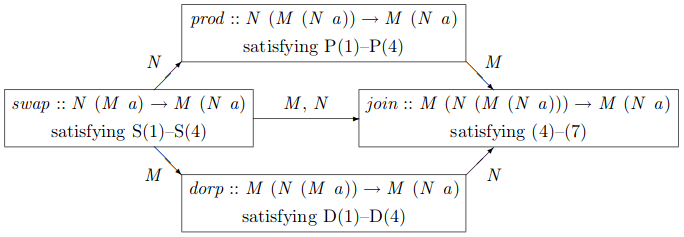
\includegraphics[width=\linewidth]{./img/graph_1}
  \label{fig:graph_1}
\end{figure}
Il secondo descrive la relazione per passare da monadi ai tre costruttori.
Questa volta gli archi descrivono proprietà richieste per ottenere il costrutto.
\begin{figure}[H]
  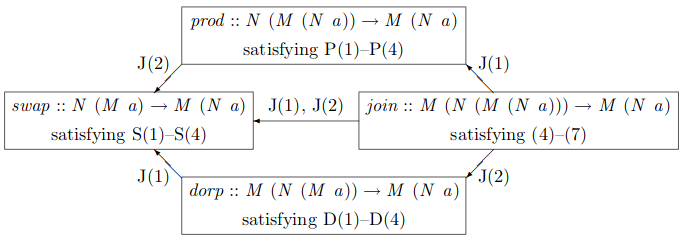
\includegraphics[width=\linewidth]{./img/graph_2}
  \label{fig:graph_2}
\end{figure}

% General Framework for Composition
\pagebreak
\section{General Framework for composition}
\label{general_framework_for_composition}

In questa sezione verranno definite una serie di classi per la generazione di
un framework per la composizione di monadi.
Dal precedente capitolo \ref{composing_monads}, definiremo una serie di classi e
funzioni per poter tipare correttamente le operazioni necessarie e definire
finalmente il tipo di dato astratto per la composizione generalizzata.
Le classi saranno implementate in sintassi Gofer per permettere di essere
codificate in un qualsiasi linguaggio funzionale.\newline

Abbiamo già visto come non sia possibile definire la composizione che riceva
due $Monads$ arbitrari.
La prossima migliore opzione è di fissare uno dei due componenti (della
composizione) e permettere all'altro componente di variare dentro ad una
famiglia di differenti Monads.
Come questo accada sarà mostrato con qualche esempio nella sezione
\ref{some_examples}, prima definiamo il framework.\newline

\subsection{Representing Functors, Premonads and Monads}
Vediamo velocemente come si rappresentano i tipi costruttori base.
\begin{align*}
  \classdef{\bm{class}\ Functor\ f\ \bm{where}}
  map &:: (a \to b) \to (f\ a \to f\ b)\\\\
  \classdef{\bm{class}\ Functor\ m \Rightarrow Premonad\ m\ \bm{where}}
  unit &:: a \to m\ a\\\\
  \classdef{\bm{class}\ Premonad\ m \Rightarrow Monad\ m\ \bm{where}}
  join &:: m\ (m\ a) \to m\ a
\end{align*}
Con $\implies$ si intende la relazione di $subtyping$, ovvero la classe a sinistra
di $\implies$ è sotto classe di quella definita a sinistra.

\subsection{Composition Construction}
\label{composition_construction}

Per descrivere la composizione di $Functors$ e $Premonads$ utilizziamo le
definizioni
\begin{align*}
  mapC &:: (Functor\ f,\ Functor\ g) \implies (a \to b) \to
  (f \ (g \ a) \to f\ (g\ b))\\
  mapC &= map\ .\ map\\
  unitC &= (Premonad\ f,\ Premonad\ g) \implies a \to f\ (g\ a)\\
  unitC &= unit\ .\ unit
\end{align*}
Queste due firme sono del tipo corretto per essere utilizzate come definizione
di funtore e premonade.
Tuttiavia, non possono essere utilizzate direttamente come istanze di funtore (e
premonade) dato che non c'è modo di definire una classe $(f\ .\ g)$ istanza
di $Functor$ o $Premonad$ o $Monad$.
Precisamente, non c'è nulla nel tipo dell'espressione $f\ (g\ x)$ che indichi
a quale costruzione è destinato.
Per evitare questa ambiguità, definiamo un costruttore $c$ per ogni
\textit{composition constructions} con l'intenzione che $c\ f\ g\ x$ sia la
composizione $f\ (g\ a)$, identificando quindi la costruzione utilizzata.
\label{composer}
\begin{align*}
  \classdef{\bm{class}\ Composer\ c\ \bm{where}}
  open &:: c\ f\ g\ x \to f\ (g\ x)\\
  close &:: f\ (g\ x) \to c\ f\ g\ x
\end{align*}
Ora proceidamo a definire le istanze di $Functor$ e $Premonad$ per i tipi compositi
, nota che queste definizioni sono \textit{general purpose}, quindi non necessitano di essere
ridefinite ogni volta.
\begin{align*}
  \classdef{\bm{instance}\ (Composer\ c\,\ Functor\ f,\ Functor\ g) \implies Functor\ (c\ f\ g)\  \bm{where}}
  map\ f &= close\ .\ mapC\ f\ .\ open\\
  \classdef{\bm{instance}\ (Composer\ c\,\ Premonad m,\ Premonad n)}
  \classdef{\implies Premonad\ (c\ m\ n)\  \bm{where}}
  unit &= close\ .\ unitC
\end{align*}
Le prossime definizioni saranno utilizzate molteplici volte nelle sezioni
seguenti.
Il loro scopo è di convertire funzioni per il $join$ di composizioni nella forma
equivalente usando un'istanza $c$ della classe $Composer$.
\begin{align*}
  wrap &:: (Composer\ c, Functor\ m, Functor\ n) \implies\\
       &\quad (m\ (n\ (m\ (n\ a))) \to m\ (n\ a)) \to\\
       &\qquad (c\ m\ n\ (c\ m\ n\ a) \to c\ m\ n\ a)\\
  wrap\ j &= close\ .\ j\ .\ mapC\ open\ .\ open
\end{align*}
In special modo le prossime due funzioni servono a fornire un modo per racchiudere
la computazione di un componente dentro il \textit{composite monad}.
\label{left_and_right}
\begin{align*}
  right &:: (Composer\ c,\ Premonad\ f) \implies g\ a \to c\ f\ g\ a\\
  right &= close\ .\ unit\\\\
  left &:: (Composer\ c,\ Functor\ f,\ Premonad\ g) \implies f\ a \to c\ f\ g\ a\\
  left &= close\ .\ map\ unit
\end{align*}

\subsection{Programming Prod Construction}
\label{programming_prod_construction}
Creaiamo un'istanza del $Composer$ sopra definito per il costruttore $prod$
\begin{align*}
  \classdef{\bm{data}\ PComp\ f\ g\ x\ =\ PC\ (f\ (g\ x))}
  \classdef{\bm{instance}\ Composer\ PComp\ \bm{where} }
  open\ (PC\ x)\ &= x\\
  close &= PC
\end{align*}
La costruzione richiede lei stessa la funzione $prod$ come definita
\begin{align*}
  \classdef{\bm{class}\ (Monad\ m,\ Premonad\ n) \implies PComposable\ m\ n\ \bm{where}}
  prod &:: n\ (m\ (n\ a)) \to m\ (n\ a)
\end{align*}
Notiamo come le richieste imposte specifichino per $n$ solamente l'appartenenza
alla classe dei $Premonads$, mentre per $m$ si richiede di essere un $Monads$
\begin{align*}
  joinP &:: (Pcomposable\ m\ n) \implies m\ (n\ (m\ (n\ a))) \to \ (n\ a)\\
  joinP &= join\ .\ map\ prod
\end{align*}
Finalmente possiamo definire che $PComp$ sia un $Monad$
\begin{align*}
  \classdef{\bm{instance}\ PComposable\ m\ n \implies Monad\ (PComp\ m\ n)\ \bm{where}}
  join &= wrap\ joinP
\end{align*}

\subsection{Programming Dorp Construction}
\label{programming_dorp_construction}
Come per il caso precedente, procediamo in maniera simile.
Creaiamo un'istanza del $Composer$ sopra definito per il costruttore $dorp$
\begin{align*}
  \classdef{\bm{data}\ DComp\ f\ g\ x\ =\ DC\ (f\ (g\ x))}
  \classdef{\bm{instance}\ Composer\ DComp\ \bm{where} }
  open\ (DC\ x)\ &= x\\
  close &= DC
\end{align*}
La costruzione richiede lei stessa la funzione $dorp$ come definita
\begin{align*}
  \classdef{\bm{class}\ (Premonad\ m,\ Monad\ n) \implies DComposable\ m\ n\ \bm{where}}
  dorp &:: m\ (n\ (m\ a)) \to m\ (n\ a)
\end{align*}
Notiamo come le richieste imposte specifichino per $m$ solamente l'appartenenza
alla classe dei $Premonads$, mentre per $n$ si richiede di essere un $Monads$
\begin{align*}
  joinD &:: (DComposable\ m\ n) \implies m\ (n\ (m\ (n\ a))) \to \ (n\ a)\\
  joinD &= join\ .\ map\ dorp
\end{align*}
Finalmente possiamo definire che $DComp$ sia un $Monad$
\begin{align*}
  \classdef{\bm{instance}\ DComposable\ m\ n \implies Monad\ (DComp\ m\ n)\ \bm{where}}
  join &= wrap\ joinD
\end{align*}

\subsection{Programming Swap Construction}
\label{programming_swap_construction}
Anche questo costruttore molto simile ai casi precedenti.
Creaiamo un'istanza del $Composer$ sopra definito per il costruttore $swap$
\begin{align*}
  \classdef{\bm{data}\ SComp\ f\ g\ x\ =\ SC\ (f\ (g\ x))}
  \classdef{\bm{instance}\ Composer\ SComp\ \bm{where} }
  open\ (SC\ x)\ &= x\\
  close &= SC
\end{align*}
La costruzione richiede lei stessa la funzione $swap$ come definita
\begin{align*}
  \classdef{\bm{class}\ (Premonad\ m,\ Monad\ n) \implies SComposable\ m\ n\ \bm{where}}
  swap &:: n\ (m\ a) \to m\ (n\ a)
\end{align*}
Notiamo come le richieste imposte specifichino sia per $m$ che per $n$ l'appartenenza
alla classe dei $Monads$, diversamente dai casi precedenti
\begin{align*}
  joinS &:: (SComposable\ m\ n) \implies m\ (n\ (m\ (n\ a))) \to \ (n\ a)\\
  joinS &= map\ join\ .\ join\ .\ map\ swap
\end{align*}
Finalmente possiamo definire che $SComp$ sia un $Monad$
\begin{align*}
  \classdef{\bm{instance}\ SComposable\ m\ n \implies Monad\ (SComp\ m\ n)\ \bm{where}}
  join &= wrap\ joinS
\end{align*}
Inoltre possiamo notare come un $SComposable$ sia egli stesso un $PComposable$ e
$DComposable$, questa definizione mostra come un costruttore $prod$ e $dorp$
possa sempre essere derivato da una definizione di $swap$
\begin{align*}
  \classdef{\bm{instance}\ SComposable\ m\ n \implies PComposable\ m\ n\ \bm{where}}
  prod &= map\ join\ .\ swap\\
  \classdef{\bm{instance}\ SComposable\ m\ n \implies DComposable\ m\ n\ \bm{where}}
  dorp &= map\ join\ .\ swap\\
\end{align*}

\subsection{Some Examples}
\label{some_examples}

\subsubsection*{Reader}
Il Monade $Reader$ è un costruttore del tipo $(r\ \to)$ che mappa per ogni tipo
$a$ alla funzione del tipo $r \to a$, la sua strutture  è definita come segue

\begin{align*}
  \classdef{\bm{instance}\ Functor\ (r \to)\ \bm{where}}
  map\ f\ g\ &= f\ .\ g\\
  \classdef{\bm{instance}\ Premonad\ (r \to)\ \bm{where}}
  unit\ x\ y\ &= x\\
  \classdef{\bm{instance}\ Monad\ (r \to)\ \bm{where}}
  join\ f\ x\ &= f\ x\ x\\
\end{align*}
Questo caso combineremo un qualsiasi Monade $n$ con il monade $Reader$ usando il
costruttore $dorp$
\begin{align*}
  \classdef{\bm{instance}\ DComposable\ (r \to)\ n\ \bm{where}}
  dorp\ m\ r\ &=\ [\ g\ r\ |\ g \leftarrow m\ r\ ]
\end{align*}

\subsubsection*{Writer}
Il \textit{Writer Monad} invece è un Monade che descrive programmi che producono
sia valori che output in maniera parallela.
Inoltre questo Monade assume che il parametro fisso $s$ sia un $Monoid$, vedi
sezione \ref{monoid}.
\begin{align*}
  \classdef{\bm{instance}\ Functor\ (Writer\ s)\ \bm{where}}
  map\ f\ (Result\ s\ a)\ &= Result\ s\ (f\ a)\\
  \classdef{\bm{instance}\ Monoid\ s \implies Premonad\ (Writer\ s)\ \bm{where}}
  unit\ &= Result\ zero\\
  \classdef{\bm{instance}\ Monoid\ s \implies Monad\ (Writer\ s)\ \bm{where}}
  join\ (Result\ s\ (Result\ t\ x)) &= Result\ (add\ s\ t)\ x\\
\end{align*}
Questo Monade è un esempio di come si utilizza il costrutto $swap$ per combinare
un qualsiasi Monade
\begin{align*}
  \classdef{\bm{instance}\ SComposable\ (Writer\ s)\ n\ \bm{where}}
  swap\ (Result\ s\ m) &=\ [\ Result\ s\ a\ |\ a \leftarrow m\ ]
\end{align*}


\subsubsection*{Maybe}
Il \textit{Maybe Monad} invece è un Monade che descrive programmi che producono
non sempre valori corretti.
Molto simile al monade $Error$.
\begin{align*}
  \classdef{\bm{instance}\ Functor\ Maybe\ \bm{where}}
  map\ f\ (Just\ x)\ &= Just\ (f\ x))\\
  map\ f\ (Nothing)\ &= Nothing\\
  \classdef{\bm{instance}\ Premonad\ Maybe\ \bm{where}}
  unit\ &= Just\\
  \classdef{\bm{instance}\ Monad\ Maybe\ \bm{where}}
  join\ (Just\ m) &= m\\
  join\ Nothing &= Nothing\
\end{align*}
Questo Monade è un esempio di come si utilizza il costrutto $prod$ per combinare
un qualsiasi Monade
\begin{align*}
  \classdef{\bm{instance}\ PComposable\ m\ Maybe\ \bm{where}}
  prod\ (Just\ m) &=\ m\\
  prod\ Nothing &=\ [\ Nothing\ ]\\
\end{align*}

\pagebreak

% Composed Monad Interpreter
\section{Composed Monad Interpreter}
\label{composed_monad_interpreter}

Ora riprendiamo il semplice interprete definito nella sezione
\ref{monadic_evaluator}, definiamolo però in termini di monade combinato.
Ricordando che la funzione di valutazione dovrà gestire l'accesso a variabili
dentro ad un $enviroments$, potrebbe produrre dell'output e richiede la gestione
degli errori.
Questo capitolo fa affidamento alle ricerche di Steele\cite{steele0},
Hughes\cite{hughes0} e Jones\cite{jones_b0}.
Tutto questo è coperto dalla seguente definizione di dato astratto:
\begin{align*}
  \bm{type}\ M\ a\ =\ Env\ \to Writer\ [String]\ (  Error\ a)
\end{align*}
Questa definizione può essere espressa nel seguente modo come composizione tra
monadi
\begin{align*}
  \bm{type}\ M\ a\ =\ DComp\ (Env \to)\ (SComp\ (Writer\ [String])\ Error) a
\end{align*}
Inoltre notiamo come, utilizzando $Gofer$, questa definizione risulti "brutta"
da vedere.
Potremmo ragionevolmente aspettarci di poter definire $M$ il una maniera migliore.
In un contesto adatto potremmo definire $M$ in maniera del tutto equivalente nel
seguente modo
\begin{align*}
  M\ a\ =\ (Env\ \to)\ .\ Writer\ [String]\ .\ Error\ a
\end{align*}
Utilizzando le funzioni \textit{general purpose} $left$ e $right$, vedi sezione
\ref{left_and_right}, possiamo includere la computazione di ogni componente dentro
all'intero $Monad M$ composto.
\begin{align*}
  inError &:: Error\ a \to M\ a\\
  inError &= right\ .\ right\\\\
  inReader &:: (Env \to a) \to M\ a\\
  inReader &= left\\\\
  inWriter &:: Writer\ [String]\ a \to M\ a\\
  inWriter &= right\ .\ left
\end{align*}
Possiamo anche notare da queste definizioni che si espone un concetto di associatività
all'interno di $M$, ossia l'operatore di composizione associa a destra.
Quindi le funzioni per accedere alla posizione del proprio monade all'interno di
$M$ devono percorre l'albero generato dalla composizione fino al proprio nodo.\\

La definizione di $eval$ è definita da
\begin{align*}
  eval &:: Expr \to M\ Value\\
  eval\ (Const\ v) &= [unit\ v]\ (\text{in maniera equivalente}\ [[v]])\\
  eval\ (Var\ n) &= [x\ |\ r \leftarrow inReader\ (lookup\ n),\ x \leftarrow inError\ r]\\
  eval\ (e_0 + e_1) &= [x+y\ |\ x \leftarrow eval\ e_0,\ y \leftarrow eval\ e_1]\\
  eval\ (Trace\ m\ e) &= [x\ |\ x \leftarrow eval\ e,\\
                      &\qquad\quad () \leftarrow inWriter\ (Result\ [m \doubleplus "=" \doubleplus x]\ ())]
\end{align*}

Osserviamo come questa versione sia finalmente la soluzione preferibile.
Propone un codice elegante e difficilmente si incorre il rischio di commettere
errori.

% Summary
\section{Summary}
\label{summary}

Ora invece cerchiamo di capire dato un $ADT$
\footnote{Abstract Data Type, tipo di dato astratto}, come potremmo comporlo con
altri monadi.
Definiamo quindi una struttura generale per gli $ADT$, notiamo prima qualche
osservazione per restringere la costruzione di questi tipi di dato astratti
\begin{itemize}
  \item Non faremo distinzioni tra coppie e sequenze in quanto un $ADT$ definito
    mediante coppia e uno mediante sequenza sono equivalenti
    \begin{align*}
      \bm{data}\ A\ a = A\ (a,\ b_1,\ \dots\ ,\ b_n) \equiv \bm{data}\ B\ a = B\ a\ b_1\ \dots\ b_n
    \end{align*}
    Con i parametri $b_1,\ \dots\ ,b_n$ fissati, è facile vedere come in ogni situazione
    in cui necessito di $A$ possa utilizzare $B$ data la funzione biettiva di conversione
    \begin{align*}
      \gamma &:: A \to B\\
      \gamma\ (A\ (x,\ y_1,\ \dots\ ,\ y_n)) &= B\ x\ y_1\ \dots\ \ y_n\\
      \gamma^{-1}\ (B\ x\ y_1\ \dots\ \ y_n) &= A\ (x,\ y_1,\ \dots\ ,\ y_n)
    \end{align*}
  \item Ogni $ADT$ sarà unario per semplicità. Nota come questa non sia una restrizione
    ma solamente una semplificazione, in quanto, ogni construttore non unario
    può essere $curryfied$ e diventarlo.
    Considerando semplicemente un parametro alla volta.
\end{itemize}
La struttura che ho trovato più generale possibile per caratterizzare tutti i tipi
di $ADT$ è la seguente
\begin{align*}
  \bm{data}\ A\ a = A_0\ a{_0}{^*}\ |\ \dots\ |\ A_n\ a{_n}{^*}
\end{align*}
Dove:
\begin{itemize}
  \item $A_i$ descrivono i vari costruttore utilizzati, inoltre $|\ A_i\ \forall i\ | >0$
    non può esistere il caso in cui un tipo di dato astratto non abbia nessun costruttore
  \item $a{_i}{^*}$ è una lista di parametri (anche vuota), $\forall i,\ k.\ a{_i}{^k}$ è $a$ oppure un tipo fissato
\end{itemize}
Notiamo come i principali $ADT$ incontrati fino ad ora rispettino questa caratterizzazione:
\begin{alignat*}{2}
  Maybe\ a &= Just\ a\ &&|\ Nothing\\
  A\ a &= A_0\ a\ &&|\ A_1 \\\\
  Error\ s\ a &= Raise\ s\ &&|\ Return\ a\\
  B\ a &= A_0\ s\ &&|\ A_1\ a\\\\
  (s \to)\ a &= Reader\ (s \to a)\\
  A\ a &= A_0\ C\ a\\\\
  ZipList\ a &= Z\ [\ a\ ]\\
  A\ a &= A_0\ D\ a
\end{alignat*}
Con $B$, $C$ e $D$ definiti come:
\begin{itemize}
  \item $B \equiv (A\ a_0)$ con $a_0$ che diventa parametro fissato
  \item $C \equiv (s \to)$ per descrivere le realzioni
  \item $D \equiv \lambda x \to [\ x\ ]$ per rappresentare l'operatore di $binding$ per liste
\end{itemize}

Definiamo inoltre il \textbf{tipo di dato astratto base}, ovvero un $ADT$ che non può essere
scomposto in altri $ADT$ di inferiore struttura.
In altri termini, un $ADT$ base non è rappresentabile mediante la composizione di
più $ADT$ in ogni sua parte.\newline

  Dato quindi un $ADT$ \textbf{base} possiamo
  \begin{itemize}
    \item pre-comporlo \footnote{$A$ pre-composto a $m$ se intendo la composizione di $m\ .\ A$}
     ad $m$, utilizzando il costruttore $prod$, se $m$ dispone di una funzione di aggregazione
     oppure se in $A$ non ci sono multiple apparizioni di $a$ parametro
    \item post-comporlo \footnote{$A$ post-composto a $m$ se intendo la composizione di $A\ .\ m$}
     ad $m$, utilizzando il costruttore $dorp$, se $m$ dispone di una funzione di aggregazione
     oppure se in $A$ non ci sono multiple apparizioni di $a$ parametro
    \item pre-comporlo utilizzando il costruttore $swap$, richiedendo all'arbitrario
      monade di possedere la proprietà commutativa
  \end{itemize}

Dare una dimostrazione formale di queste proprietà richiede l'esistenza di funzioni
ausiliarie di commutazione che porterebbero alla costruzione di $prod$ e $dorp$, la cui
esistenza porterebbe alla definizione di $join$.
Non stiamo quindi concludendo che due monadi qualsiasi sono componibili tra di loro
dato che in questa lista riassuntiva richiediamo sempre di essere a conoscenza della
struttura di almeno uno dei due monadi.
Difatti stiamo solo ristrutturando in maniera equivalente le conclusioni del capitolo
\ref{general_framework_for_composition}.\\
Inoltre non sempre la composizione di due monadi è la modalità preferibile di composizione,
nella sezione \ref{state_transformer} vediamo un caso in cui la composizione
è semanticamente diversa al monade che stiamo cercando.

\vfill

\appendix
\pagebreak
\section{Proofs}
\label{proofs}

\subsection{Exception is a Monad}
\label{exception_is_a_monad}
Dimostriamo che il tipo astratto $Exception$ \ref{exceptions} è un
\textit{Functor}, \textit{Premonad} e \textit{Monad}\newline

\textbf{Dim:}\newline

Dimostriamo che il tipo astratto con le operazioni di \textit{map},
\textit{unit} e \textit{join} rispetta le leggi definite per \textit{Functor},
\textit{Premonad} e \textit{Monad}, $M1\dots7$

\begin{align*}
  \textbf{data}\ Exception\ a &= Raise\ String\ |\ Return\ a \\\\
  map &:: (a \to b) \to Exception\ a \to Exception\ b\\
  map\ f\ (Raise\ s) &= Raise\ s\\
  map\ f\ (Return\ x) &= Return\ (f\ x)\\\\
  unit &:: a \to Exception\ a\\
  unit &= Return\\\\
  join &:: Exception\ (Exception\ a) \to Exception\ a\\
  join\ (Raise\ s) &= Raise\ s\\
  join\ (Return\ x) &= x
\end{align*}

Per la dimostrazione procedo per casi sui costrutti $Raise$ e $Return$

\begin{framed}
  \begin{align*}
      (Raise)\qquad
      &\quad map\ id\ (Raise\  s) && \{map\}\\
      =&\quad (Raise\ s) && \{id^{-1}\}\\
      =&\quad id\ (Raise\ s)\\\\
      (Return)\qquad
      &\quad map\ id\ (Return\ x) && \{map\}\\
      =&\quad Return\ (id\ x) && \{id\}\\
      =&\quad Return\ x
    %\caption*{$(M1)$}
  \end{align*}

  \begin{align*}
      (Raise)\qquad
      &\quad (map\ f\ .\ map\ g)\ (Raise\ s) && \{composition\}\\
      =&\quad map\ f\ (map\ g\ (Raise\ s)) && \{map\}\\
      =&\quad map\ f\ (Raise\ s) && \{map\}\\
      =&\quad Raise\ s && \{map^{-1}\}\\
      =&\quad map\ (f\ .\  g)\ (Raise\ s)\\\\
      (Return)\qquad
      &\quad (map\ f\ .\ map\ g)\ (Return\ s) && \{composition\}\\
      =&\quad map\ f\ (map\ g\ (Return\ s)) && \{map\}\\
      =&\quad map\ f\ (Return\ (g\ s)) && \{map\}\\
      =&\quad Return\ (f\ (g\ s)) && \{composition^{-1}\}\\
      =&\quad Return\ ((f\ .\ g)\ s) && \{map^{-1}\}\\
      =&\quad map\ (f\ .\  g)\ (Return\ s)
    %\caption*{$(M2)$}
  \end{align*}

  \begin{align*}
      (Raise)\qquad
      &\quad (unit\ .\ f)\ (Raise\ s) && \{composition\}\\
      =&\quad unit\ (f\ (Raise\ s)) &&\{unit\}\\
      =&\quad Return\ (f\ (Raise\ s)) && \{map^{-1}\} \\
      =&\quad map\ f\ (Return\ (Raise\ s)) && \{unit^{-1}\} \\
      =&\quad map\ f\ (unit\ (Raise\ s)) && \{composition^{-1}\} \\
      =&\quad (map\ f\ .\ unit)\ (Raise\ s)\ \\\\
      (Return)\qquad
      &\quad (unit\ .\ f)\ (Return\ s) && \{composition\}\\
      =&\quad unit\ (f\ (Return\ s)) &&\{unit\}\\
      =&\quad Return\ (f\ (Return\ s)) && \{unit^{-1}\} \\
      =&\quad Return\ (f\ (unit\ s)) && \{composition^{-1}\} \\
      =&\quad Return\ ((f\ .\ unit)\ s) && \{map^{-1}\} \\
      =&\quad (map\ f\ .\ unit)\ (Return\ s)\
    %\caption*{$(M3)$}
  \end{align*}

  \begin{align*}
      (Raise)\qquad
      &\quad (join\ .\ map\ (map\ f))\ (Raise\ s) && \{composition\}\\
      =&\quad join\ (map\ (map\ f)\ (Raise\ s)) && \{map\}\\
      =&\quad join\ (Raise\ s)  && \{join\}\\
      =&\quad Raise\ s\ && \{map^{-1}\}\\
      =&\quad map\ f\ (Raise\ s) && \{join^{-1}\}\\
      =&\quad map\ f\ (join\ (Raise\ s)) && \{composition^{-1}\}\\
      =&\quad map\ f\ .\ join\ (Raise\ s)\\\\
      (Return)\qquad
      &\quad (join\ .\ map\ (map\ f))\ (Return\ s) && \{composition\}\\
      =&\quad join\ (map\ (map\ f)\ (Return\ s)) && \{map\}\\
      =&\quad join\ (Return\ (map\ f\ s))  && \{join\}\\
      =&\quad map\ f\ s && \{join^{-1}\} \quad(*)\\
      =&\quad map\ f\ (join\ (Return\ s)) && \{composition^{-1}\}\\
      =&\quad map\ f\ .\ join\ (Return\ s)\
    %\caption*{$(M4)$}
  \end{align*}
  \begin{align*}
      (Raise)\qquad
      &\quad (join\ .\ unit)\ (Raise\ s) && \{composition\}\\
      =&\quad join\ (unit\ (Raise\ s)) && \{unit\}\\
      =&\quad join\ (Return\ (Raise\ s)) && \{join\}\\
      =&\quad Raise\ s && \{id^{-1}\}\\
      =&\quad id\ (Raise\ s) \\\\
      (Return)\qquad
      &\quad (join\ .\ unit)\ (Return\ s) && \{composition\}\\
      =&\quad join\ (unit\ (Return\ s) && \{unit\}\\
      =&\quad join\ (Return\ (Return\ s) && \{join\}\\
      =&\quad Return\ s && \{id^{-1}\}\\
      =&\quad id\ (Return\ s)
    %\caption*{$(M5)$}
  \end{align*}

  \begin{align*}
      (Raise)\qquad
      &\quad (join\ .\ map\ unit)\ (Raise\ s)) && \{composition\}\\
      =&\quad join\ (map\ unit\ (Raise\ s)) && \{map\}\\
      =&\quad join\ (Raise\ s) && \{join\}\\
      =&\quad Raise\ s\ && \{id^{-1}\}\\
      =&\quad id\ (Raise\ s) \\\\
      (Return)\qquad
      &\quad (join\ .\ map\ unit)\ (Return\ s) && \{composition\}\\
      =&\quad join\ (map\ unit\ (Return\ s)) && \{map\}\\
      =&\quad join\ (Return\ (unit\ s)) && \{unit^{-1}\}\\
      =&\quad join\ (unit\ (unit\ s)) && \{composition^{-1}\}\\
      =&\quad join\ .\ unit\ (unit\ s) && \{M5\}\\
      =&\quad id\ (unit\ s) && \{unit\}\\
      =&\quad id\ (Return\ s)
    %\caption*{$(M6)$}
  \end{align*}

  \begin{align*}
      (Raise)\qquad
      &\quad (join\ .\ map\ join)\ (Raise\ s)) && \{composition\}\\
      =&\quad join\ (map\ join\ (Raise\ s)) && \{map\}\\
      =&\quad join\ (Raise\ s) && \{join^{-1}\}\\
      =&\quad join\ (join\ (Raise\ s)) && \{composition^{-1}\}\\
      =&\quad join\ .\ join\ (Raise\ s) \\\\
      (Return)\qquad
      &\quad (join\ .\ map\ join)\ (Return\ s) && \{composition\}\\
      =&\quad join\ (map\ join\ (Return\ s)) && \{map\}\\
      =&\quad join\ (Return\ (join\ s)) && \{join\}\\
      =&\quad join\ s && \{join^{-1}\}\quad(*)\\
      =&\quad join\ (join\ (Return\ s)) && \{composition^{-1}\}\\
      =&\quad join\ .\ join\ (Return\ s)
    %\caption*{$(M7)$}
  \end{align*}
\end{framed}

Osservazione $(*)$, utilizzando la definizione inversa di $join$ richiedo che il suo
parametro $s$ sia di tipo $s::Exception$

% ------------------------------------------------------------------------------

\pagebreak
\subsection{Natural Join doesn't exist}
\label{natural_join_doesn_t_exist}
Dimostriamo che non esiste il $join$ naturale tra \textit{Monads} generici
\ref{conditions_for_composition}.
In parole, è impossibile costruire la funzione $join$ per la composizione di due
$Monads$ utilizzando esclusivamente gli operatori dei monadi.\\
Supponiamo di lavorare con due $Monads$ dati $M$ e $N$.
Nel caso più generale un termine ben tipato può essere costruito utilizzando
solo gli operatori $map$, $unit$ e $join$.
Precisamente possiamo costruire solo termini generati dalla seguenti regole
\begin{align*}
  \begin{split}
    a \overset{id}{\longrightarrow} a
  \end{split}
    \begin{split}
      \frac
        {b \overset{f}{\longrightarrow} c\quad a \overset{g}{\longrightarrow} b}
        {a \overset{f\ .\ g}{\longrightarrow} c}
    \end{split}
  % \end{split}
\end{align*}
\begin{align*}
  \begin{split}
    \frac
      {a \overset{f}{\longrightarrow} b}
      {M\ a \overset{map_M\ f}{\longrightarrow} M\ b}
  \end{split}
  \begin{split}
    \frac
      {a \overset{f}{\longrightarrow} b}
      {N\ a \overset{map_N\ f}{\longrightarrow} N\ b}
  \end{split}
\end{align*}
\begin{align*}
  \begin{split}
    a \overset{unit_M}{\longrightarrow} M\ a
  \end{split}
  \begin{split}
    a \overset{unit_N}{\longrightarrow} N\ a
  \end{split}
\end{align*}
\begin{align*}
  \begin{split}
    M\ (M\ a) \overset{join_M}{\longrightarrow} M\ a
  \end{split}
  \begin{split}
    N\ (N\ a) \overset{join_N}{\longrightarrow} N\ a
  \end{split}
\end{align*}
Queste regole comprendono il più piccolo set per poter modellare adeguatamente
le operazioni in maniera naturale.
Utilizzando questa caratterizzazione mostrerò che non c'è modo di costruire un
termine del tipo $M\ (N\ (M\ (N\ a))) \to M\ (N\ a)$ e quindi che non esiste il
$join$ naturale per la composizione dei \textit{Monads}.\newline

Per convenienza utilizzerò le seguenti convenzioni:
\begin{itemize}
  \item scriverò la stringa $MNMNX$ al posto dell'espressione $M\ (N\ (M\ (N\ X)))$
        ,inoltre per l'i-esimo elemento di una qualsiasi stringa $X$ utilizzerò
        la notazione $(X)_i$, ad esempio, $(MNMMX)_1 = M$, $(MNMMX)_5 = X$ e $(MNMMX)_6 = \emptyset$
  \item userò la notazione $rd\ X$ per la stringa ottenuta rimuovendo tutti i
        duplicati adiacenti da $X$, per esempio, $rd\ MMNMNNX\ =\ MNMNX$
  \item $\req{X}$ è l'operatore che ritorna $|rd\ X|$, ossia la cardinalità di $rd\ X$

\end{itemize}
Notiamo quindi che se le regole base definissero solo funzioni del tipo
\begin{align*}
  X \to Y \implies
  \begin{cases}
   \req{X}\ <\ \req{Y} &if\ (X)_1 \neq (Y)_1\\
   \req{X}\ \leq\ \req{Y} &if\ (X)_1 = (Y)_1
  \end{cases}
  && (*)
\end{align*}
allora potremmo conseguire che la funzione $join$ non è ottenibile essendo che
la funzione del tipo $MNMNX \to MNX$ ha come proprietà
\begin{align*}
  (MNMNX)_1 = M = (MNX)_1 \land
  \req{MNMNX}\ >\ \req{MNX}
\end{align*}
E quindi non rispetta $(*)$.\newline

\textbf{Dim:}\newline

Procedo per induzione sull'altezza $h$ dell'albero di derivazione generato dalle
regole definite.\newline

\textbf{Caso base:} $(h = 0)$ nessuna regola mi permette di procedere
senza eseguire almeno un passo quindi il predicato $X \to_0 Y$ è falso.
Implica che la proprietà $(*)$ è vacuamente vera.\newline

\textbf{Caso induttivo:} $(h \to h+1)$\\
La proprietà $(*)$ da dimostrare diventa quindi
\begin{align*}
  X \to_{h+1} Y \implies
  \begin{cases}
   \req{X}\ <\ \req{Y} &if\ (X)_1 \neq (Y)_1\\
   \req{X}\ \leq\ \req{Y} &if\ (X)_1 = (Y)_1
  \end{cases}
  && (**)
\end{align*}
L'ipotesi induttiva invece è così definita
\begin{align*}
  X \to_{\leq h} Y \land (X)_1 \neq (Y)_1 \implies \req{X}\ <\ \req{Y} &&(IP1)\\
  X \to_{\leq h} Y \land (X)_1 = (Y)_1 \implies \req{X}\ \leq\ \req{Y} &&(IP2)
\end{align*}
Procedo per casi per ogni regola definita
\begin{itemize}
  \item \textbf{[id]}
    \begin{align*}
        \frac{\req{X}\ \leq\  \req{X}}{X \overset{id}{\longrightarrow}_{h+1} X}
    \end{align*}
      In questo caso è ovvio che $(X)_1 = (X)_1$\\
      E dato che l'operatore $\leq$ gode della proprietà riflessiva quindi ho
      dimostrato $(**)$ per l'identità
  \item \textbf{[composition]}
    \begin{align*}
        \frac{
        \exists Z.
        \quad \overset{(1)}{Z \overset{f}{\longrightarrow}_{\leq h} Y}
        \quad \overset{(2)}{X \overset{g}{\longrightarrow}_{\leq h} Z}
        }{X \overset{f\ .\ g}{\longrightarrow}_{h+1} Y}
    \end{align*}
    Procediamo per casi su $(1)$ e $(2)$:
    \begin{itemize}
      \item $(Z)_1 = (Y)_1 \land (X)_1 = (Z)_1$, quindi applico l'ipotesi induttiva
        $(IP2)$ a $(1)$ e $(2)$ e ottengo che $\req{Z}\ \leq\ \req{Y} \land
        \req{X}\ \leq\ \req{Z}$.\\
        Dato che l'operatore $\leq$ gode della proprietà
        riflessiva ho che vale quindi $\req{X}\ \leq\ \req{Y}$.\\
        Per concludere basta osservare che $(Z)_1 = (Y)_1 \land (X)_1 = (Z)_1
        \implies (X)_1 = (Y)_1$ e quindi devo provare la proprietà $\req{X}\ \leq\ \req{Y}$
        in $(**)$.\\
      \item $(Z)_1 = (Y)_1 \land (X)_1 \neq (Z)_1$, quindi applico l'ipotesi induttiva
        $(IP2)$ a $(1)$ e $(IP1)$ a $(2)$ e ottengo che $\req{Z}\ \leq\ \req{Y} \land
        \req{X}\ <\ \req{Z}$.\\
        Concatenando $(1)$ e $(2)$ ottengo $\req{X}\ <\ \req{Z}\ \leq\ \req{Y}$
        che implica $\req{X}\ <\ \req{Y}$.\\
        Per concludere basta osservare che $(Z)_1 = (Y)_1 \land (X)_1 \neq (Z)_1
        \implies (X)_1 \neq (Y)_1$ e quindi devo provare la proprietà $\req{X}\ <\ \req{Y}$
        in $(**)$.\\
      \item $(Z)_1 \neq (Y)_1 \land (X)_1 = (Z)_1$, duale al caso precedente.\\
      \item $(Z)_1 \neq (Y)_1 \land (X)_1 \neq (Z)_1$, quindi applico l'ipotesi induttiva
        $(IP1)$ a $(1)$ e $(2)$ e ottengo che $\req{Z}\ <\ \req{Y} \land
        \req{X}\ <\ \req{Z}$.\\
        Dato che l'operatore $<$ gode della proprietà
        riflessiva ho che vale quindi $\req{X}\ <\ \req{Y}$.\\
        Ho concluso dimostrando $(**)$ dato che senza interessarci a quanto vale
        l'uguaglianza tra $(X)_1$ e $(Y)_1$ ho comunque già valida l'ipotesi più
        forte, ovvero $\req{X}\ <\ \req{Y}$.\\
    \end{itemize}
    Per tutti i quattro casi vale $(**)$ quindi ho dimostrato $(**)$ per la composizione.
    \item \textbf{[map]} dimostro per $map_M$ e ottengo anche il duale $map_N$
      \begin{align*}
          \frac{
            \overset{(1)}{X \overset{f}{\longrightarrow}_{\leq h} Y}
          }{MX \overset{map_M\ f}{\longrightarrow}_{h+1} MY}
      \end{align*}
      Ora notiamo che vale $(MX)_1 = M = (MY)_1$ quindi la proprietà da dimostrare
      in tutti i casi è la meno restrittiva, ossia $\req{MX} \leq\ \req{MY}$.\\
      Procedo per casi su $(1)$:
      \begin{itemize}
        \item $(X)_1 = (Y)_1$, quindi applico l'ipotesi induttiva $(IP2)$ e
          ottengo $\req{X}\ \leq\ \req{Y}$.\\
          Ora mi trovo davanti a due sottocasi:
          \begin{itemize}
            \item $(X)_1 = M (\implies (Y)_1 = M)$, allora ho che
              \begin{align*}
              \req{MX} = \req{MMX'} = \req{MX'} = \req{X}\\
              \req{MY} = \req{MMY'} = \req{MY'} = \req{Y}
              \end{align*}
              quindi data l'ipotesi induttiva ottengo che
            \begin{equation*}\req{MX} = \req{X} \leq_{ip. ind}\ \req{Y} = \req{MY}\end{equation*}
            \item $(X)_1 = N (\implies (Y)_1 = N)$, allora ho che
              \begin{align*}
              \req{MX} = \req{MNX'} \overset{(a)}{=} 1 + \req{NX'} = 1 + \req{X}\\
              \req{MY} = \req{MNY'} \overset{(a)}{=} 1 + \req{NY'} = 1 + \req{Y}
              \end{align*}
              quindi data l'ipotesi induttiva ottengo che
            \begin{equation*}\req{MX} = 1 + \req{X} \leq_{ip. ind}\ 1 + \req{Y} = \req{MY}\end{equation*}
              Il passaggio $(a)$ è giustificato dal fatto che $\req{MNX'} = |rd\ MNX'| = 1 + |rd\ NX'|$
          \end{itemize}
        \item $(X)_1 \neq (Y)_1$, quindi applico l'ipotesi induttiva $(IP1)$ e
          ottengo $\req{X}\ <\ \req{Y}$.\\
          Ora mi trovo davanti a due sottocasi:
          \begin{itemize}
            \item $(X)_1 = M (\implies (Y)_1 = N)$, allora ho che
              \begin{align*}
              \req{MX} = \req{MMX'} = \req{MX'} = \req{X}\\
              \req{MY} = \req{MNY'} = 1 + \req{NY'} = 1 + \req{Y}
              \end{align*}
              quindi data l'ipotesi induttiva ottengo che
            \begin{equation*}\req{MX} = \req{X} <_{ip. ind}\ \req{Y} <\ 1 + \req{Y} = \req{MY}\end{equation*}
            \item $(X)_1 = N (\implies (Y)_1 = M)$, allora ho che
              \begin{align*}
              \req{MX} = \req{MNX'} = 1 + \req{NX'} = 1 + \req{X}\\
              \req{MY} = \req{MMY'} = \req{MY'} = \req{Y}
              \end{align*}
              quindi data l'ipotesi induttiva ottengo che
            \begin{align*}
              &\quad\req{MX} = 1 + \req{X} <_{ip. ind}\ 1 + \req{Y}\\
              &\implies 1 + \req{X} \leq\ \req{Y} = \req{MY}
            \end{align*}
          \end{itemize}
          Concludo quindi di aver dimostrato $(**)$ per l'operatore $map$.
      \end{itemize}
      \item \textbf{[unit]} dimostro per $unit_M$ e ottengo anche il duale $unit_N$
        \begin{equation*}X \overset{unit_M}{\longrightarrow_{h+1}} MX\end{equation*}
        Mi trovo davanti a due casi:
        \begin{itemize}
          \item $(X)_1 = M \implies \req{MX} = \req{MMX'} = \req{MX'} = \req{X}$\\
            Per riflessività di $\leq$ ottengo
            \begin{equation*}\req{X} = \req{MX} \leq\ \req{MX}\end{equation*}
            Inoltre essendo che $(X)_1 = M = (MX)_1$ allora ho dimostrato $(**)$
            per questo caso.
          \item  $(X)_1 = N \implies \req{MX} = \req{MNX'} = 1 + \req{NX'} = 1 + \req{X}$\\
            Quindi ottengo
            \begin{equation*}\req{X} <\ 1 + \req{X} = \req{MX}\end{equation*}
            Inoltre essendo che $(X)_1 = N \neq M = (MX)_1$ allora ho dimostrato $(**)$
            per questo caso.
        \end{itemize}
        Concludo quindi di aver dimostrato $(**)$ per l'operatore $unit$.
      \item \textbf{[join]} dimostro per $join_M$ e ottengo anche il duale $join_N$
        \begin{equation*}MMX \overset{join_M}{\longrightarrow_{h+1}} MX\end{equation*}
        Per l'operatore di $join$ concludo direttamente osservando le due proprietà
        \begin{align*}
          (MMX)_1 = M = (MX)_1\\
          \req{MMX} = \req{MX} \leq\ \req{MX}
        \end{align*}
        Quindi concludo anche per quest'ultimo caso che la proprietà $(**)$ è valida
        per l'operatore di $join$.
\end{itemize}

Questa dimostrazione prova quindi che, con la grammatica sopra definita,
la funzione $join$ non è ottenibile essendo funzioni del tipo $MNMNX \to MNX$
hanno come proprietà
\begin{align*}
  (MNMNX)_1 = M = (MNX)_1 \land
  \req{MNMNX}\ >\ \req{MNX}
\end{align*}
Non ottenibili in questo contesto dato che non soddisfano $(*)$.\newline


\textbf{Conseguenze:} come conseguenze possiamo notare che gli operatori $map$ e
$unit$ possono essere generati in quanto rispettano $(**)$
\begin{align*}
  (MNX)_1 = M = (MNX)_1\  \land\  &\req{MNX} \leq \req{MNX} &&(map_M\ .\ map_N\ f)\\
  &\req{X} < \req{MNX} &&(unit_M\ .\ unit_N)
\end{align*}
Mentre nessuno tra $prod$, $dorp$ e $swap$ può essere costruito.
% ------------------------------------------------------------------------------

\pagebreak
\subsection{Monad Comprehensions Equivalence}
\label{monad_comprehensions_equivalence}
Dimostriamo la seguente proprietà, mostrata nella sezione \ref{monad_comprehensions}
\begin{align*}
    &{[\ v_0 + v_1\ |\ v_0 \leftarrow eval\ e_0\ env,\ v_1 \leftarrow eval\ e_1\ env\ ]} = \\
    &bind\ (eval\ e_0\ env) (\lambda\ v_0 \to bind\ (eval\ e_1\ env) (\lambda\ v_1 \to unit (v_0 + v_1)))
\end{align*}

Per semplicità utilizzerò le seguenti definizioni durante la dimostrazione,
essendo equazioni non modifico la semantica della proprietà da dimostrare

\begin{align*}
    E_i = eval\  e_i\  env \qquad \forall i \in {[0,\ 1]}
\end{align*}
La proprietà da dimostrare diventa
\begin{align*}
    &{[\ v_0 + v_1\ |\ v_0 \leftarrow E_0,\ v_1 \leftarrow E_1\ ]} = \\
    &bind\ E_0\ (\lambda\ v_0 \to bind\ E_1\ (\lambda\ v_1 \to unit\ (v_0 + v_1)))
\end{align*}

\textbf{Dim:}\newline

Prima di cominciare bisogna definire una regola che segue direttamente da
un'osservazione delle regole $(M5)$ e $(M6)$
\begin{align*}
    map\ (f\ .\ unit)\ &=\ map\ f\ .\ unit \qquad&& (Sub)
  \end{align*}
Questa proprietà si prova facilmente con la seguente dimostrazione
\begin{framed}
\begin{align*}
    &\quad map\ (f\ .\ unit)\ && \{M2\}\\
    =&\quad map\ f\ .\ map\ unit &&\{(*)\}\\
    =&\quad map\ f\ .\ unit
\end{align*}

\begin{align*}
    (*)\ join\ .\ unit\ \stackrel{(M5)}{=} id \stackrel{(M6^{-1})}{=} join\ .\ map\ unit\\
    \Rightarrow unit\ =\ map\ .\ unit
\end{align*}


Ora invece possiamo procedere alla dimostrazione principale
\begin{align*}
    &\quad{[\ v_0 + v_1\ |\ v_0 \leftarrow E_0,\ v_1 \leftarrow E_1\ ]} && \{joinComp\}\\
    =&\quad join\ {[\ {[\ v_0 + v_1\ |\ v_1 \leftarrow E_1\ ]}\ |\ v_0 \leftarrow E_0 \ ]} && \{mapComp\}\\
    =&\quad join\ {[\ map\ (v_0+)\ E_1\ |\ v_0 \leftarrow E_0 \ ]} && \{mapComp\}\\
    =&\quad join\ (map\ (\lambda\ v_0 \to\\
     &\quad \qquad map\ (v_0+)\ E_1)\ E_0 ) && \{id\}\\
    =&\quad join\ (map\ (\lambda\ v_0 \to\\
     &\quad \qquad (map\ (v_0+)\ .\ id)\ E_1)\ E_0 ) && \{M5^{-1}\}\\
    =&\quad join\ (map\ (\lambda\ v_0 \to\\
     &\quad \qquad (map\ (v_0+)\ .\ join\ .\ unit)\ E_1)\ E_0 ) && \{M4^{-1}\}\\
    =&\quad join\ (map\ (\lambda\ v_0 \to\\
     &\quad \qquad (join\ .\ map\ (map\ (v_0+))\ .\ unit)\ E_1)\ E_0 ) && \{Sub\}\\
    =&\quad join\ (map\ (\lambda\ v_0 \to\\
     &\quad \qquad (join\ .\ map\ (map\ (v_0+)\ .\ unit))\ E_1)\ E_0 ) && \{M4^{-1}\}\\
    =&\quad join\ (map\ (\lambda\ v_0 \to\\
     &\quad \qquad (join\ .\ map\ (unit\ .\ (v_0+)))\ E_1)\ E_0 ) && \{composition\}\\
    =&\quad join\ (map\ (\lambda\ v_0 \to\\
     &\quad \qquad join\ (map\ (unit\ .\ (v_0+))\ E_1))\ E_0 ) && \{bind^{-1}\}\\
    =&\quad join\ (map\ (\lambda\ v_0 \to\\
     &\quad \qquad bind\ E_1\ (unit\ .\ (v_0+)))\ E_0 ) && \{bind^{-1}\}\\
    =&\quad bind\ E_0\ (\lambda\ v_0 \to bind\ E_1\ (unit\ .\ (v_0+))) && \{composition\}\\
    =&\quad bind\ E_0\ (\lambda\ v_0 \to bind\ E_1\ (\lambda\ v_1 \to unit\ (v_0+v_1))) && \{E_0\ e\ E_1\}\\
    =&\quad bind\ (eval\ e_0\ env) \lambda\ v_0 \to \\
     &\quad \qquad \qquad bind\ (eval\ e_1\ env) \lambda\ v_1 \to \\
     &\quad \qquad \qquad \qquad unit\ (v_0+v_1)
  \end{align*}
\end{framed}

\pagebreak
\section{State Transitions}
\label{state_transitions}

In questa sezione mostro il motivo per cui non sempre la composizione ha
l'effetto sperato.
Il $Monad$ per lo $State\ transitions$ difatti rappresenta un esempio pratico
in cui, dato un $Monad\ M$, la composizione generalizzata non è ciò che ci
aspettiamo.\newline

L'$ADT$ per lo $state\ transitions$
\begin{align*}
  \bm{data}\ State\ s\ a = ST(s \to (a,\ s))
\end{align*}
Difatti il monade per le transizioni di stato è definito
\begin{align*}
  \classdef{\bm{instance}\ Functor\ (State\ s)\ \bm{where}}
  map\ f\ (ST\ x)\ &= ST(\lambda s \to \bm{let}\ (s',\ x) = st\ s\ \bm{in}\ (s',\ f\ x))\\
  \classdef{\bm{instance}\ Premonad\ (State\ s)\ \bm{where}}
  unit\ x &= ST(\lambda s \to (s,\ x))\\
  \classdef{\bm{instance}\ Monad\ (State\ s)\ \bm{where}}
  join\ (ST\ m) &= ST(\lambda s \to \bm{let}\ (s',\ ST\ m') = m\ s\ \bm{in}\ m'\ s')\\
\end{align*}
Possiamo notare come lo $State$ possa essere definito in termini di
\textit{Monad Composition} tra $Reader$ e $Writer$.
Difatti possiamo comporre lo $State$ in questo modo, $State\ s\ a = (s \to)\ .\ (Writer\ s)\ a$.
Oppure mediante il framework della sezione \ref{general_framework_for_composition},
$\bm{data}\ State\ s\ a = DComp\ (s \to)\ (Writer\ s)\ a$.\newline

Questo nuovo $Monad$ non è equivalente allo $State$ definito sopra, difatti nel caso
$unit$ il monade composto ritorna, dato un qualsiasi $s$ lo $zero$ del $Monoid$
$s$, inoltre richiede appunto che $s$ sia $Monoid$.\newline

Potremmo quindi creare un caso specifico per combinare un qualsiasi $Monad$ con
lo \textit{State Transitions}, prima di tutto definiamo il suo tipo, sarà generico
in $m$
\begin{align*}
  \bm{data}\ StateM\ m\ s\ a = STM(s \to m\ (a,\ s))
\end{align*}
Poi istanziamolo ad essere un monade
\begin{align*}
  \classdef{\bm{instance}\ Monad\ m \implies Functor\ (StateM\ m\ s)\ \bm{where}}
  map\ f\ (STM\ xs)\ &= STM(\lambda s \to [(s',\ f\ x)\ |\ (s',\ x) \leftarrow xs\ s])\\
  \classdef{\bm{instance}\ Monad\ m \implies Premonad\ (StateM\ m\ s)\ \bm{where}}
  unit\ xs &= STM(\lambda s \to [(s,\ x)])\\
  \classdef{\bm{instance}\ Monad\ m \implies Monad\ (StateM\ m\ s)\ \bm{where}}
  join\ (STM\ xss) &= STM(\lambda s \to [(s'',\ x)\ |\ (STM\ xs,\ s') \leftarrow xss\ s, \\
                   &\qquad\qquad\qquad\qquad\qquad\qquad(s'',\ x) \leftarrow xs\ s'])\\
\end{align*}
Ora riusciamo a comporre un qualsiasi $Monads$ con il sistema di \textit{State Transitions}
, notiamo però che abbiamo creato un sistema di composizione generalizzata ad hoc.
Quindi non sfruttiamo il framework precedentemente creato.\newline

Una spiegazione a questo fatto è che la composizione di monadi generata dal
nostro framework non riesce ad esprimere la relazione che intercorre tra i
componenti del monade composto.
Questa spiegazione, istanziata al nostro caso, in particolare non esprime
l'equivalenza tra il parametro in input al $Reader\ Monad$ con l'output prodotto
nel $Writer\ Monad$.\newline

Steele \cite{steele0}, prova a definire un meccanismo generico anche per gli $ADT$
che hanno queste caratteristiche di relazioni tra monadi composti.
Utilizza un sistema di pseudomonadi per riuscire a comporre monadi lasciando il monade
arbitrario non più ai "lati" della composizione ma al "centro", non approfondirò
questo punto all'interno di questo report.

\section{Monoid}
\label{monoid}

Un \textit{Monoid} è un tipo di dato astratto definito dalla seguente
dichiarazione di classe

\begin{figure}[H]
  \centering
  \footnotesize % adapt to your page size
  \begin{align*}
  \noalign{\textbf{class}\ Monoid\ s\  \textbf{where}}
  zero &:: s\\
  add &:: s \to s \to s
  \end{align*}%
\end{figure}

Dato che nel contesto di questo report un \textit{Monoid} può essere utilizzato
esclusivamente per operare sui \textit{Monads} richiedo che $add$ sia
associativa a destra e sinistra con $zero$.
Possibili \textit{Monoid} sono le liste, le funzioni e i numeri interi

\begin{figure}[H]
  \centering
  \footnotesize % adapt to your page size
  \begin{align*}
  \noalign{\textbf{instance}\ Monoid\ [a]\  \textbf{where}}
  zero &=\ [\ ]\\
  add &=\  (\doubleplus)\\\\
  \noalign{\textbf{instance}\ Monoid\ (a $\to$ a)\  \textbf{where}}
  zero &=\  id\\
  add &=\  ( . )\\\\
  \noalign{\textbf{instance}\ Monoid\ Int\  \textbf{where}}
  zero &=\  0\\
  add &=\ (+)
  \end{align*}%
\end{figure}

\pagebreak
\section{Scala Code}
\label{scala_code}
Come richiesto in questa sezione inserirò degli $snippets$ di codice $Scala$
per la composizione generalizzata di monadi.
Non essendo pratico di $scala$ sono ricorso agli esempi definiti da Omura \cite{omura0}
e Milewski \cite{milewski0}.
Questo esempio ricrea il framework generalizzato per la composizione simile a quello
visto nella sezione \ref{general_framework_for_composition}.

\begin{lstlisting}[style=myScalastyle, caption=Functor and Monad Traits]
  trait Functor[F[_]]{
    def map[A,B](ma:F[A])(f:(A) => B):F[B]
  }
  // per l'esempio unisco la definizione di Monad e Premonad
  trait Monad[M[_]] extends Functor[M]{
    def unit[A](a:A):M[A]
    // come il join operator
    def flatten[A](mm:M[M[A]]):M[A]
    // flatMap puo' essere utile negli esempi pratici
    // derivata da map e join
    def flatMap[A,B](ma:M[A])(f:(A)=>M[B]) = flatten(map(ma)(f))
  }
\end{lstlisting}

Per l'esempio considererò una coppia di monadi composta con il costruttore $swap$,
vedi sezione \ref{swap_construction}

\begin{lstlisting}[style=myScalastyle, caption=Swap Constructor]
  trait SComposable[M[_],N[_]]{
    def M:Monad[M]
    def N:Monad[N]
    def swap[A](nm:N[M[A]]):M[N[A]]
  }
\end{lstlisting}

Definiamo qualche istanza di $Monad$

\begin{lstlisting}[style=myScalastyle, caption=Type class instances]
implicit val OptionMonad = new Monad[Option]{
  def map[A, B](ma: Option[A])(f: (A) => B) = ma.map(f)
  def unit[A](a: A) = Option(a)
  def flatten[A](mm: Option[Option[A]]) = mm.flatMap(identity)
}
implicit val ListMonad = new Monad[List]{
  def map[A, B](ma: List[A])(f: (A) => B) = ma.map(f)
  def unit[A](a: A) = List(a)
  def flatten[A](mm: List[List[A]]) = mm.flatten
}
\end{lstlisting}
\pagebreak
Definiamo anche la sintassi per $map$ e $flatmap$ per le monadi scala, essenzialmente
serve per poterle utilizzare dentro al ciclo $for$.
\begin{lstlisting}[style=myScalastyle, caption=Composer]
case class Mval[M[_]:Monad,A](v:M[A]){
  def map[B](f:(A)=>B) = implicitly[Monad[M]].map(v)(f)
  def flatMap[B](f:(A)=>M[B])
    = implicitly[Monad[M]].flatMap(v)(f)
}
implicit def v2M[M[_]:Monad, A](v:M[A]) = Mval(v)
def compose[M[_],N[_],A](mna:M[N[A]])
  (implicit mn:Monad[({type MN[x] = M[N[x]]})#MN])
  :Mval[({type MN[x] = M[N[x]]})#MN,A]
  = Mval[({type MN[x] = M[N[x]]})#MN,A](mna)
\end{lstlisting}
Quindi passiamo a definire istanze di $SComposable$ come $Monad$

\begin{lstlisting}[style=myScalastyle, caption=SComposable is Monad]
implicit def monadSCompose[M[_],N[_]]
  (implicit m:Monad[M], n:Monad[N], s:SComposable[M,N])
  = new Monad[({type MN[x] = M[N[x]]})#MN]{
    def map[A,B](ma:M[N[A]])(f: (A) => B)
      = m.map(ma)(n.map(_)(f))
    def unit[A](a: A) =  m.unit(n.unit(a))
    def flatten[A](mnmn:M[N[M[N[A]]]])
      = m.map(m.flatten(m.map(mnmn)(s.swap(_))))(n.flatten(_))
}
\end{lstlisting}

Ora definiamo la composizione generalizzata mediante $swap$ per le due istanze
definite
\begin{lstlisting}[style=myScalastyle, caption=Composing List]
  implicit def MonadListSComposable[M[_]]
    (implicit monadM:Monad[M])
    = new SComposable[M,List] {
    def M = monadM
    def N = implicitly[Monad[List]]
    def swap[A](nm: List[M[A]]):M[List[A]] = nm match {
      case List() => monadM.unit(List())
      case x::xs => for {
          y <- x;
          ys <- swap(xs)
        } yield y::ys
    }
  }
\end{lstlisting}
\pagebreak
\begin{lstlisting}[style=myScalastyle, caption=Composing Optional]
  implicit def MonadOptionSComposable[M[_]]
    (implicit monadM: Monad[M])
    = new SComposable[M,Option]{
      def M = monadM
      def N = implicitly[Monad[Option]]
      def swap[A](nm: Option[M[A]]) = nm match{
        case Some(ma) => monadM.map(ma)(Option(_))
        case None => monadM.unit(None)
      }
  }
\end{lstlisting}

Per finire concludo con la definizione di un semplice main per testare il codice
appena scritto
\begin{lstlisting}[style=myScalastyle, caption=Main]
  // outputs: List(Some(4), Some(5), Some(8), Some(9))
  println(for {
      i<- compose(List(Option(1), None, Option(5)))
      j<- compose(List(Option(3), Option(4)))
    } yield i+j)

  // outputs: Some(List(4, 5, 8, 9))
  println(for {
      i<- compose(Option(List(1, 5)))
      j<- compose(Option(List(3, 4)))
    } yield i+j)
\end{lstlisting}


% Bibliography:
\clearpage
\begin{thebibliography}{99}
  \bibitem{jones0} M. P. Jones, L. Duponcheel, \emph{Composing Monads*}, Research Report YALEU/DCS/RR-1004, December 1993
  \bibitem{walder0} P. Walder, \emph{Mathematical Structures in Computer Science}, Nice, France, June 1994
  \bibitem{walder1} P. Walder, \emph{Monads fo functional programming}, University of Glasgow, Scotland
  \bibitem{steele0} L. Steele, \emph{Building Interpreters by Composing Monads}, Thinking Machines Corporation, Cambridge, Massachusetts
  \bibitem{hughes0} J. Hughes, \emph{Why Functional programming Matters}, The University, Glasgow
  \bibitem{jones_b0} L. P. Jones, D. R. Lester, \emph{Implementing Functional Languages: a tutorial}, University of Glasgow, University of Manchester
  \bibitem{milewski0} Bartosz Milewski, \url{https://github.com/typelevel/CT_from_Programmers.scala/tree/master/src/main/tut}
  \bibitem{omura0} Shingo Omura, \url{https://github.com/everpeace/composing-monads}
\end{thebibliography}

\end{document}